% !TeX spellcheck = en_US
% !TeX encoding = UTF-8

% COMPILE WITH:
% `latexmk`
% You need lualatex and biber (in all TeXLive distributions)

\documentclass[
    numbers=noenddot,
    %listof=totoc,
    parskip=half-,
    fontsize=12pt,
    paper=a4,
    oneside,
    titlepage,
    bibliography=totoc,
    chapterprefix=false,
%    draft
]{scrbook}

% use lualatex or xelatex
%\usepackage{fontspec}
\usepackage{graphicx}
\usepackage[onehalfspacing]{setspace}

% better language support
%\usepackage{polyglossia}
%\setdefaultlanguage{english}
%\setotherlanguage{german}

\usepackage{tocbasic}
\usepackage{booktabs}
\usepackage{multicol}
\usepackage{multirow}
\usepackage{amsmath}

\usepackage[]{scrlayer-scrpage}
\usepackage{hyperref}

% \usepackage[autostyle,english=american,german=quotes]{csquotes}
\usepackage[linesnumbered,ruled]{algorithm2e} % this is to write algorithms, if you do not like it, the other options are algorithmic, or pseudocode

% better bibliography (biblatex style)
% use biber to compile
\usepackage[style=numeric, sorting=none, backend=biber, language=english, backref=true, maxcitenames=2]{biblatex}

% better quotes
% use \enquote{text}
\usepackage[autostyle,english=american,german=quotes]{csquotes}
\addbibresource{bibliography.bib}

% appendix
\usepackage[titletoc]{appendix}

% where to put all images and figures
\graphicspath{{images/}}

% YOUR PACKAGES


% Title
\title{Health Status for Hard Drive Failure Detection}

% Author
\author{Miguel Vieira Pereira}

% Date
\date{\today}

% CHOOSE ACCORDINGLY
%\newcommand{\thesisType}{Bachelorarbeit}
\newcommand{\thesisType}{Masterarbeit}

\makeatletter
\let\thetitle\@title
\let\theauthor\@author
\let\thedate\@date
\makeatother

\pagestyle{scrheadings}

\begin{document}

%%%%%%%%%%%%%%%%%%%%%%%%%%%%%%%%%%%%%%%%%%%%%%%%%%%%%%%%%%%%%%%%%%%%%%%%%%%%%%%%%%%%%%%%%
\frontmatter
% !TeX spellcheck = en_US
% !TeX encoding = UTF-8
\begin{titlepage}
    \centering
    \begin{onehalfspace}
    	
        	
\includegraphics[width=7cm]{uni-logo.png}\\
        	\vspace{1.0cm}
        	\large {\bfseries Lehrstuhl das Fach Verteilte Informations und Multimedia-Systeme}\\

        	\vspace{2.5cm}

            \begin{doublespace}
            	{\textsf{\Huge{\thetitle}}}
            \end{doublespace}

        	\vspace{2cm}

            \Large{Masterarbeit von}\\

        	\vspace{1cm}

        	{\bfseries \large{\theauthor}}

        	\vfill

        	{\large
        		\begin{tabular}[l]{cc}
        			\textsc{1.~Pr\"ufer} & \textsc{2.~Pr\"ufer} \\
        			Prof.~Dr.~Harald Kosch & Prof.~Dr.~Michael Granitzer
        		\end{tabular}
        	}

        	\vspace{1.5cm}

        	\parbox{\linewidth}{\hrule\strut}

            \vfill

	    \thedate
    \end{onehalfspace}
\end{titlepage}


\tableofcontents
\newpage

% -- ABSTRACT
% !TeX spellcheck = en_US
% !TeX encoding = UTF-8
\chapter*{Abstract}

Users require an increasingly amount of storage in order to allow the multitude of online service available nowadays.
As the number and size of data centers increases, so does the need of automated tools for their maintenance.
In particular, in order to prevent data loss and to ensure the reliability of the service hardware failures need to be predicted.

Most of the hardware failures in such systems occur on the hard drive.
As a consequence, vendors introduced a set of values that allow these disks to be monitored: the SMART attributes.
Many machine learning based approaches have been proposed to detect problems with the disks before they fail and the data on them becomes unrecoverable.

In the current work, we present some of the state of the art methods to tackle the problem of hard drive failure prediction.

Additionally, we leverage the fact that the sequence of SMART attributes samples of a disk form a time series in order to improve existing methods.
We use the concept of health status in which the gradual deterioration of a hard drive is taken account and, consequently, the samples in the training set can be classified in multiple classes, not only ``Healthy'' or ``Failing''.

In order to take further advantage of the time series aspect we implement, to the best of our knowledge, the first Long Short-Term Memory model to tackle the hard drive failure prediction problem using its SMART attributes.
Also four other state of the art models are implemented and extended to deal with the health status version of the problem.


\textbf{Keywords:} Hard drive failure prediction, SMART, health status, neural networks, recurrent neural networks, long short-term memory 
\newpage

% -- Acknowledgements (optional)
% % !TeX spellcheck = en_US
% !TeX encoding = UTF-8
\chapter*{Acknowledgments}

% I would first like to thank my thesis advisor ...
% \newpage

% -- List of figures
\thispagestyle{empty}
\cleardoublepage
\listoffigures
\newpage

% -- List of tables
\thispagestyle{empty}
\cleardoublepage
\listoftables
\newpage

%%%%%%%%%%%%%%%%%%%%%%%%%%%%%%%%%%%%%%%%%%%%%%%%%%%%%%%%%%%%%%%%%%%%%%%%%%%%%%%%%%%%%%%%%
\mainmatter

% -- Chapters
% following IMRaD structure
% adjust for your liking
\chapter{Introduction}\label{chap:introduction}

\section{Motivation}\label{sec:motivation}

The amount of information produced and processed in the world has seen a steady increase over the past decades.
The world internet traffic is increasing exponentially since a few decades.
Edholm's Law\cite{Edholm04} predicts that this behaviour should continue until at least 2030.
It shows that telecommunications data rates are rising in a manner analogous to the one predicted by Moore's Law\cite{Moore98}: doubling every $18$ months.
Even 20 years after this prediction was done, it is still used by organizations responsible by developing the infrastructure to transmit huge amount of data \cite{Mammela17}.

As the amount of data generated by users all around the world increases, the need to store and access this data increases accordingly.
This evolution is matched by an expansion on the number of digital services offered to users: musics, videos, books and other types of files and media that can be accessed from anywhere.
The solution companies found to these problems was Cloud Computing.
Even though Cloud Computing is a vague term, one way to define it is "a technique where IT services are provided by massive low-cost computing units connected by IP networks"\cite{Qian09}.

However, even though Cloud Computing is sold as a way for users to access computing resources they don't have physical access to, the hardware responsible for this computing power must be placed somewhere.
This is achieved by the establishment of multiple data centers all around the world to which devices from anywhere can connect in order to get access to the desired services.
Microsoft, for example, has 300 data centers worldwide to provide their services to their clients\cite{MicrosoftDataCenters}.

A data center is a complex installation that consists of thousands of hard drives connect by kilometers of optical fiber cables.
Therefore, there are massive amounts of investment done in order to create and maintain these facilities.
Microsoft is investing \$80 billion in order to improve their data centers\cite{MicrosoftDataCenters}.
So there is a demand for services related to the maintenance and improvement of data centers.

In this context, one of the main aspects of Cloud Computing in general is the strong virtualization and reliability of the system\cite{Qian09}, meaning that even if some of the hardware fails the service should still be provided without interruption.
So, as hardware components fail, they need to be replaced to ensure that the system keeps working for a long time.

Moreover, in order to maintain a reliable system it is not enough to only replace the hardware after it fails.
In order to prevent some serious issues such as data loss without having to permanently have a copy of all the data it is necessary to predict the hardware failures.

Therefore, one of the main problems faced by data centers is the need to detect which pieces of hardware are going to fail before a fatal crash occurs to allow it to be replaced.
This allows both the prevention of data loss.

Out of all the components that are part of a computer, $80\%$ of the failures occur due to the problems on the hard drives, as indicated by Table \ref{devicefailuretable}
Therefore, there is a special focus on predicting failures on disks.

\begin{table}
    \begin{center}
      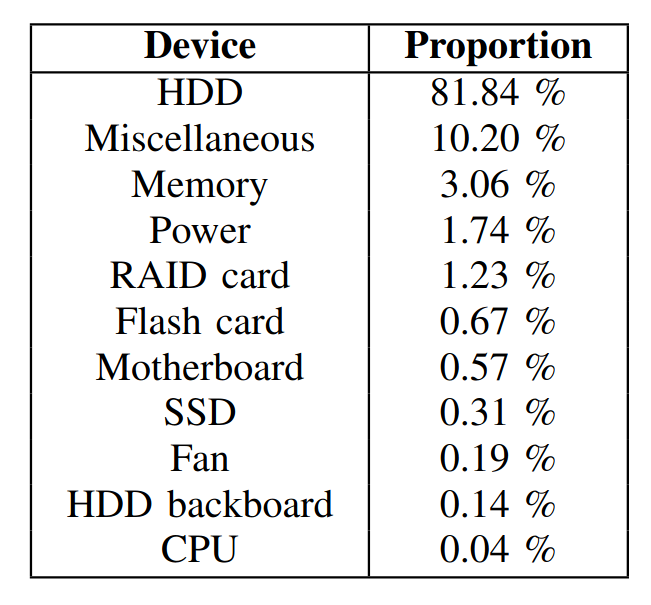
\includegraphics[width=.6\linewidth]{FailureProportions.png}
      \caption[Failure percentage by component]{Data center failure percentage by component - \cite{Wang17}}
      \label{devicefailuretable}
    \end{center}
  \end{table}

Hardware vendors are well aware of this situation and the difficulties related to managing thousands of hard drives.
So, in order to allow their users to better tackle these problems, they added a monitoring system to their drives.
This technology is called SMART (Self-Monitoring, Analysis, and Reporting Technology).

Using this protocol, vendors can provide to users indicators of the disk status to the user.
Some of these attributes are Power-On Hours, Air Flow Temperature and Reallocated Sector Count (number of sectors that had to be copied elsewhere on the disk after a failed read or write operation in order to prevent data loss)\cite{SamsungSSD}.

The SMART system can also include status of different attributes.
However, these are limited to threshold not exceeded or threshold exceeded for each attribute, where the threshold is a reference value set by the vendor\cite{SamsungSSD}.

Moreover, even when there is an indication that a threshold has been exceeded, it does not mean that the drive will suffer an unrecoverable failure.
Sometimes it can be a sign that the drive will work more slowly than its specifications indicate.

In addition to that, these status provided by the vendors consider each attribute independently.
They do not take into account the fact that some problems in the hard drive can cause different indicators to increase simultaneously, so by considering the relationship between different attributes would allow problems to be more accurately detected.
For example, having a huge number of Power-On cycles when compared to Power-On hours may indicate a problem in the disk that causes it to crash and restart constantly.

Finally, this ad-hoc approach uses static values and do not consider the evolution of the attributes over time.
Imagine the situation of a disk that has not reallocated any disks so far, and suddenly rate at which sectors have to be reallocated increases.
By taking into account how this attribute evolves over time, this problem can be more quickly detected before the threshold value is reached.

However, even though the built-in failure detection system is not very effective, it doesn't mean that the data itself cannot be used to obtain more interesting results, after all the problem of failure detection must still be solved.
Current research uses mostly machine learning approaches such as SVMs and Neural Networks to tackle this problem.
Further details of how these methods work will be detailed in \hyperref[chap:background]{Chapter 2}. 
% TODO: give a link to the chapter about the current research

This project has three main objectives.
The first one is to create a library that implement some of the current approaches used in research.
The idea is to also made it in such a way that it can be extended with new methods in order to allow them to be easily tested and compared to other ones. 

After creating the library, further tests can be performed on existing methods to understand how they evolve as their parameters change.
For example, the research of Zhu et al. on backpropagation neural networks for disk failure\cite{Zhu13} uses a neural network with one single hidden layer with a fixed amount of 30 nodes on it.
With our library, we can change the number of nodes of a neural network analogous to the one presented by them and study how the results change when the number of layer or nodes is altered.

The third objective is to extend existing methods to also make use of the concept of Health Status introduced by Xu et al.\cite{Xu16}.
Their idea is to give a score from $1$ to $n$ to each sample depending on how close it is to a failure, instead of using only a pass/fail status.

So, the goal is to extend other methods to support more than two classes and study their reaction to this change.
Different models can be extended this way, whether they are other neural network based methods such as \cite{Zhu13} or even if they use other approaches such as the Random Forest one presented by Shen et al.\cite{Shen18}.  

\section{Problem}\label{sec:problem}

Let $x_{i,t}$ be the vector in which the $j^{th}$ component designs the measure of the $j^{th}$ SMART attribute for disk $i$ at time $t$.
As input, we also have a value $y_i$ that is either $0$, if this disk has eventually failed or $1$ if, until the end of the observation period, the disk kept working properly.
Also, let the number of different smart attributes be equal to $m$.

Then given a series of vectors with the SMART attributes for an unseen disk, $\hat{x}_t$, we want to output a value $\hat{y}_t$.
Here, $\hat{y}_t$ should be equal to $1$ if the algorithm predicts that the samples $\left(\hat{x}_1\dots\hat{x}_t\right)$ are closer to the samples in the input that did not fail than to the ones that malfunctioned, and $0$ otherwise.

In a real world scenario, if the value $\hat{y}_t$ is equal to $1$, then a warning should be sent to the people responsible for maintaining the data center in order to replace the concerned disk.

This corresponds to a classical classification problem.
The numerical vectors as input and a binary output suggest that machine learning methods such as Classification Trees\cite{Li14}, Support Vector Machines\cite{Zhu13} and Neural Networks\cite{Xu16} are well adapted to tackle this problem.

However, this problem has  a few specific characteristics.
First of all, the samples are not completely independent, since the values $\left(x_{i,1},x_{i,t}\right)$ are a time series that describe the status of disk $i$ through time.
As we will see on Chapter 3, this can be a motivation to use methods such as LSTM (Long Short-Term Memory) networks that can encode and work with time dependencies.
% TODO: put a link to the chapter here

Moreover, even other methods such as Random Forests that can't easily deal with time dependencies can be extended to make use of the time series aspect of the data.
This can be one by appending new components to $x_{i,t}$ corresponding to the value $x_{i,t}[j] - x_{i,t-\delta}[j], j\in\left\{1,\dots,m\right\}$.
In this case, $\delta$ is a constant that allows the algorithm to detect sudden changes in the value of an attribute\cite{Shen18}.

A second point that needs to be mentioned is that the amount of disks in each class is not similar at all.
Since a hard drive has a service life of around 3 to 5 years\cite{Vishwanath10}, and observations are performed for a few weeks, no failure will be observed for most of the disks.
The ratio of failing disks over the total amount is between $0.4\%$ and $1.9\%$\cite{Xu16}.
So, any approach to this problem has to handle this imbalance in the input data.

Thirdly, the meaning of each SMART attribute is not the same for different vendors\cite{SamsungSSD}.
The protocol is standardized, but what it reports is not.
So, an algorithm for failure prediction cannot be trained on data from different vendor disks.
Moreover, in general, it is not a good idea to mix data from different disks on the same dataset, since they can have different failure causes profiles.

Most of the time, this does not pose a problem to the datasets generated by the data centers.
This is due to the fact that, in practice, a data center uses hundreds of copies of the hardware of the same model and has at most a couple of different models.
This allows for the replacement if failing disks do be done in a cheaper and more swiftly manner, since it simplifies stock management.

% TODO: introduce the concept of time in advance
When evaluating an algorithm there are two main metrics that must be taken into account.
The first one is the FDR (Failure Detection Rate).
This is equal to the ratio between the number of disks that are correctly predicted to be failing and the total amount of failing disks.
Its value should be as close to $1$ as possible

The second metric is the FAR (False Alarm Rate).
This is equal to the ratio between the number of disks that are wrongly predicted to be failing and the total amount of disks that do not fail.
Its value should be as close to $0$ as possible.

The challenge is to find algorithms that find an equilibrium between this values.
If it predicts every $\hat{x}_t$ to give an output $\hat{y} = 1$, the FAR will be equal to $0$, but the FDR too.
On the other hand, if it predicts every $\hat{x}_t$ to give an output $\hat{y} = 0$, the FDR will be equal to $1$, but the FDR too.
So, we notice that a trade off must be done between the FDR and the FAR.

It does not mean, however, that both metrics should be treated identically.
Suppose that during a period of one month, $2\%$ of the hard drives in a data center fail.
This corresponds to a lifetime of about 4 years, which may represent a real world scenario.
If the FDR decreases by $1\%$, then only $0.02\%$ of the disks of the data center will fail without a warning during one month.

In contrast, if the FAR increases by the same amount, then $0.98\%$ of the disks of the whole data center will be unnecessarily replaced during the same period.
This is close to $50\%$ of the disks that actually need to be replaced and can incur a substantial cost.
So, most algorithms in the literature prefer to have a bias towards classifying a disk as working rather than failing.

Aditionnaly, it is impossible to reach perfect values for both indicators.
This is due to the fact that hard drives are subject to real world conditions.
For example, a short circuit on a disk may be caused by an electrical surge, but it does not depend on the internal state of the disk and thus cannot be predicted by the approach using SMART attributes.

Some additional steps can be made after executing the machine learning algorithm.
A common one is the use a voting algorithm.
The simplest way this can be done is as follows\cite{Shen18}: each sample $\hat{x}_{t}, t\in\left\{1,\dots,T\right\}$, often including the change rate components, is evaluated independently.
A sequence $\hat{y}_t, \left\{1,\dots,T\right\}$ is obtained.
Then, a fraction $f$ is chosen.
If more than $f\cdot T$ of $\hat{y}_t$ is equal to $0$ then the output of the system is $0$, otherwise it is $1$.

The main advantage of this method is that it allows to easily control the trade off between the FDR and the FAR which can be desired as we have seen above.
It suffices to increase $f$ in order to decrease the FAR at a cost of also decreasing the FDR.

\chapter{Background}\label{chap:background}

As detailed in Section \ref{sec:problem}, the failure detection problem can be viewed as a sequence classification problem.

The first step is to develop methods to classify the samples instead of the entire sequences.
In order to do so, multiple machine learning methods are possible such as decision trees and neural networks.

In the next few sections we will discuss how these approaches were used in literature and the results that they obtained.
Moreover, for the five methods we actually implemented we will discuss the theory behind them and the motivation to use them.

\section{Decision Tree}\label{sec:decisiontree}

A decision tree represents a flowchart in the form of if-else statements.
Because of this, one of its main advantages is the fact that it is fairly easy to interpret it and to understand how it arrives at its conclusions.

Formally, a decision tree is a rooted tree $G = (V, E), E \subseteq V^2$.
The leaves of the tree are labeled with one of the possible output classes.

The other nodes are called decision nodes.
Evaluating an unseen sample, consists in traversing the tree starting from the root and taking a left or right child of the current node depending on the conditions in it until a leaf is reached, which corresponds to an output.

For the following discussion, it may be useful to have at least a superficial understanding of the training process of a decision tree.
The tree starts with a single node, the root, and all the training samples are placed there.
The root is then added to a queue.

While the queue is not empty, the first node in it is processed.
The processing step starts by choosing a splitting value $c$ for each attribute.

Then, for each attribute $i$, the samples are divided in two sets depending on whether its value is bigger or smaller than a threshold value $c_i$.
One way to obtain the threshold value is to compute the average of the attribute $i$ over the samples assigned to the node being processed.

Then the algorithm computes which of the partitions maximize a certain criterion function.
A common criterion to use here is the information gain, which is the opposite of the Shannon Entropy \cite{shannon1948mathematical}.

Then, two new nodes and edges are created.
The original node is then labeled by $(i, c_i)$ where $i$ is the index of the attribute that maximizes the criterion function.
The training samples that were assigned to the node are then split between its two children according to the value of their attribute $i$.

If some condition for one of the children is met such as it is at a certain depth or all samples in the same node belong to the same class, then the child is not added to the queue.
Instead, it is kept in the graph as a leaf with a label that corresponds to the class that appears most frequently in the samples assigned to it.
Otherwise, the node is added to the queue to be processed later.

After being trained, when the tree needs to predict the class of a certain sample $x$ it will start traversing the tree from its root. 
Then, at each non-leaf node, it will read the label $(i, c)$ and if $x_i$ is smaller than $c$ then the next node in the traversal is the left child, else it is the right child.

The training and the evaluation processes are illustrated by Algorithm \ref{algo:train-decision-tree} and Algorithm \ref{algo:test-decision-tree} respectively.

\begin{minipage}{0.92\textwidth}
    \begin{algorithm}[H]
        \caption{\textsc{TrainDecisionTree}($T$: train set)}\label{algo:train-decision-tree}
        \SetKw{KwReturn}{return} % define some custom keywords
        \SetKw{KwPrint}{print}
        \SetKw{KwNot}{not}
        \SetKw{KwTrue}{true}
        \SetKwFor{While}{while}{do}{end while}
        $r \gets Node()$, $q \gets Queue()$\;
        $r.samples \gets T$\;
        $q.push(r)$\;
        \While{\KwNot $q.empty()$} {
            $n \gets q.pop()$, $maxi \gets \infty$, $att \gets -1$\;
            $c \gets -1$\;
            \For{$i \gets 1$ \KwTo $m$} {
                $c' \gets avg(n.samples, i)$\;
                $s_1 \gets \{x \in n.samples \mid x_i \leq c'\}$\;
                $s_2 \gets \{x \in n.samples \mid x_i > c'\}$\;
                $gain = criterion(s_1, s_2)$\;
                \If{$gain > maxi$}{
                    $mini \gets gain$\;
                    $att \gets i$\;
                    $c \gets c'$\;
                    $n.left.samples \gets s_1$, $n.right.samples \gets s_2$\;
                }
            }

            $n.attribute \gets att$\;
            $n.threshold \gets c$\;
            
            \For{child of $n$}{
                \If{$shouldProcess(child)$} {
                    $q.push(child)$\;
                } \Else {
                    $child.isLeaf \gets \KwTrue$\;
                    $child.result = mostCommon(child.samples)$\;
                }
            }
        }
    \end{algorithm}
\end{minipage}

\begin{minipage}{0.92\textwidth}
    \begin{algorithm}[H]
        \caption{\textsc{EvaluateDecisionTree}($tree$: decision tree, $x$: sample)}\label{algo:test-decision-tree}
        \SetKw{KwReturn}{return} % define some custom keywords
        \SetKw{KwPrint}{print}
        \SetKw{KwNot}{not}
        \SetKw{KwTrue}{true}
        \SetKwFor{While}{while}{do}{end while}
        $cur \gets tree.root$\;
        \While{\KwNot cur.isLeaf} {
            \If{$x\left[cur.attribute\right] \leq cur.threshold$}{
                $cur \gets cur.left$\;
            } \Else {
                $cur \gets cur.right$\;
            }
        }

        \KwReturn cur.result\;
    \end{algorithm}
\end{minipage}


The explainability of this model comes from the fact that when a sample is evaluated, the decision steps that resulted in the corresponding output can be followed, as show in Algorithm \ref{algo:test-decision-tree}.
So, it is possible to verify which attributes are taken into account and to predict what would happen if one of then was changed.
Therefore, the impact of each attribute can be interpreted.

Decision trees come in two flavors: classification and regression trees.
The former corresponds to classifying samples in discrete, independent classes.
So, classification trees will treat samples from different classes as different entities.

Regression trees, on the other hand, work with outputs that are continuous, real numbers instead of discrete classes.
So, for instance, we can assign the value 0 to the training samples that represent failing disks and value 1 to the ones that denote working ones.

When evaluating an unseen sample, the output will then be a number between 0 and 1.
If this number is close to 0 then we can interpret that the regression tree predicts the sample to represent a disk in a failing state. 

The most important aspect of the differences between a classification and regression tree for us will be how to extend them to deal with more than 2 classes.
The classification tree will treat samples from different classes as independent entities.
On the other hand, regression trees will be able to identify a hierarchy between classes: a class corresponding to the value 1 is closer to the one with the value 0 than to the class we label with the value 5 for example.

The consequences of these differences and how we have tackled them are explained in our methodology in Chapter \ref{chap:methods}.

Decision trees were used by Li \textit{et al.} \cite{Li14} to tackle the hard drive failure prediction problem.
They tested both classification and regression trees.

This work introduces some additional concepts that are useful for the implementation of other methods and is actually used by later researchers.
Firstly, they add a feature selection step that keeps only a subset of the SMART features passed as input.

More interesting though is the fact that they add columns to their table corresponding to the change rate of the SMART attributes.
It allows the algorithm to take into account previous samples, even though decision trees evaluate different samples independently.

One of the key aspects of including the change rate is that it is not specific to the models they have used.
Instead, it is an approach that can be applied to improve almost any other method used to tackle this problem 

In their work, they use a voting algorithm to go from a classification of the samples to the classification of the sequence.
This way, in order to classify an unseen hard drive, they take the last $N$ samples and evaluate each of them using the decision tree.
If more than $\frac{N}{2}$ of them are put in the failing class, then the hard drive is classified as failing.

The results they obtained were promising.
They obtained FARs below 0.5\% while keeping the FDR around 95\% for the classification trees.

The regression tree model used a continuous value between $-1$ and $0$ as the health status value, linearly dependent on how much time before the breakdown of the drive the sample was taken.
This approach was able to increase the FDR by 1\% while also decreasing the FAR to be around 0.3\% when compared to the classification tree implemented by them.

\section{Backpropagation Neural Network}\label{sec:BackpropagationNeuralNetwork}

A neural network is a machine learning model that can be used to perform both classification and regression tasks.
Its name comes from the fact that its development was inspired by how a brain work: with neurons that can be interpreted as nodes and synapses that connect them.
The first implementation of this approach is credited to Rosenblatt with his Perceptron architecture \cite{rosenblatt1957perceptron}.

In general, this architecture can be represented as a sequence of layer of nodes (the neurons) and a set of directed edges from every node in layer $l$ to every node in layer $l+1$.
Moreover, the $j^{th}$ node of layer $i$ emits an output value $o^{(l)}_i$ and its connection to the $j^{th}$ node of the layer $l+1$ has weight $w^{(l+1)}_{ij}$.

The first and last layers are special.
The values of $o^{(1)}_i$ correspond to the input values to the network.
The values in these nodes represent the sample being evaluated.

The output of the last layer is the prediction done by the network.
For a regression problem, for instance, this is the value of the independent variable predicted for the given input sample.

From the values on the input layer we can compute the output values of every node in the network.
In order to do that, we need to introduce the concept of activation function.

The activation function, denoted by $\varphi$, is a non-linear function that will map the input given to a node to its output.
For the layer $l+1$, the input $u^{(l)}_i$ to its $i^{th}$ node is the sum of the output values of layer $l$ scaled by the weights of the connection.
The output of a node is the value of $\varphi\left(u^{(l)}_i\right)$.
Formally:

\begin{equation}
    \begin{cases}
        u^{(l)}_i &= \sum_{j=1}^{n}o^{(l-1)}_j w^{(l)}_{ij} \\
        o^{(l)}_i &= \varphi\left(u^{(l)}_i\right)
    \end{cases}
\end{equation}

Therefore, from an input to the first layer, we can compute the values of the outputs of the second layer.
This process can be repeated until the output value for the last layer is calculated.

The fact that the activation function takes as input a linear combination of the outputs of the nodes of the previous layer explains why it shouldn't be linear.
If $\varphi$ were linear, then the output of each neuron would be linear with respect to the outputs of the previous one.
So, the output of the last layer would be a linear function of the inputs.

Having a non-linear activation function is desired, therefore, not because otherwise the math would not work.
Instead, it is due to the fact that there are other, simpler methods to learn linear patterns such as SVM or simply the least-squares method.
The power of a neural network is exactly that it is able to recognize non-linear patterns, which can only be done when using non-linear activation functions.

Here we notice that the activation function does not need to be the same on every layer, but it does not change the analysis we are performing here.
Some of the most commonly used activation functions are the Rectified Linear Unit (ReLU) and the logistic function.

The logistic function, given by $\phi(z) = \dfrac{1}{1+e^{-z}}$, is particularly useful for the output layer of a classification problem such as the one we have.
This is because it maps values in $(-\infty, \infty)$ to $[0,1]$, which allows us to output values in a known and convenient range.

A classic interpretation of this value is the probability $p$ of the sample belonging to class labeled as 1 during training.
Trivially, the probability of the sample belonging to class 0 is $1-p$.
So, the model is able to not only classify the sample, but also to indicate how confident it is that this is the correct result.

As shown, the output value of every neuron, including the output ones, can be computed from the input values and the weights.
So, in order to fully describe a network, the only attributes that we need are the weights.
The challenge is, therefore, how to determine the weights that are appropriate for the problem at hand.

The method used by the Backpropagation Neural Network (BPNN) to compute the weights of the network is called backpropagation.
It is inspired by the Gradient Descent approach first developed by Cauchy \cite{lemarechal2012cauchy} long before the advent of computers.

The intuition behind this method is to try to explore a search space to find a point where some function is as large as possible.
It uses the fact that, the gradient of a function $g$ at a point $u$, denoted $\nabla g(u)$, is a vector that points in the direction in which the function grows the fastest at $u$.

So, the idea is to check the value of $g$ at $u + \eta \nabla g(u)$.
Here, $\eta$ is the size of the step taken and is called the learning rate.

A learning rate too high may lead us to skip some points of interest.
On the other hand, a small $\eta$ may lead to exploring too many points in a region that is not the ideal one, which slows down the process.
So, there is a tradeoff between the thoroughness of the exploration and the time it takes, which can be controlled by the learning rate.

In the context of neural networks, during training the model tries to minimize a loss function $\lambda$.
The process of finding a minimum is analogous to the one of finding a minimum, it suffices to maximize the function $-\lambda$.

The objective is to explore the space of possible weights.
In order to do so, a sample is given to the network and its output is compared to the expected result.

It can be proven \cite{amari1993backpropagation} that at each step, each weight of the network should be updated by:

\begin{equation}
\Delta w_{ij}^{(l)} = -\eta e_i^{(l)} o_{j}^{(l-1)}
\end{equation}

Where $e_i^{(l)}$ is called the error signal of the $i^{th}$ node at layer $l$.
The error signal can be computed recursively as follows \cite{amari1993backpropagation}:

\begin{equation}\label{eq:error_signal}
\begin{cases}
    e_i^{(k)} &= \varphi '(u_i^{(k)}) \\
    e_i^{(l)} &= \varphi '(u_i^{(l)}) \sum_j w_{ij}^{(l)}e_j^{(l+1)}, l \in \{1,\dots,k-1\}
\end{cases}
\end{equation}

One notable aspect of Equation \ref{eq:error_signal} is that the error signal of neurons on layer $l$ depend only on the error signals on layer $l+1$.
So, the errors for each node of a given layer can be computed in parallel.

This property is so important that the capacity of computing such values in parallel made it possible to introduce neural network training in GPUs \cite{steinkraus2005using} which was one of the main causes of the AI spring that has been happening on the last 20 years.

Zhu \textit{et al.} \cite{Zhu13} applied the backpropagation neural network approach presented above to the problem of hard drive failure detection.
The lowest FAR they obtained was 0.48\% while keeping an FDR of 94.6\%.
They were even able to obtain a model that had and FDR of 100\% on their test set, but with a relatively higher FAR of 2.26\%.

However, their work did not completely explore the potential of the model that they have used.
Specially due to the fact that they only varied one hyperparameter.
The only variable they changed on their experiment was the number of samples per failing hard drive to be used in the training and test processes.
So, if the time window was 12 hours, for example, only the samples from failing disks on the test set were only those taken on the last 12 hours before a hard drive failed.

For instance, they also included the change rates of the attributes, but they did not show by how much adding them improves their model.
Also, they manually selected the SMART attributes they used to train the model, which makes reduces the reproducibility of the experiment specially when using other datasets.

\section{Recurrent Neural Network}\label{sec:RecurrentNeuralNetwork}

A backpropagation neural network is a relatively simple yet powerful model capable of solving multiple regression \cite{suresh2015particle} and classification \cite{paola1995review} problems.
However, it can have some limitations.

The most relevant one to the problem we have at hand is that it evaluates one sample at a time.
It does not care about previous samples and does not have any type of memory.

However, in our problem the concept of sequence and, more specifically, of time series is present.
Due to how they work, backpropagation neural networks are not capable of efficiently working with sequences.

This limitation was found early on and there are works from the 1980s already trying to figure out how a neural network could store a state depending on what the previous samples were \cite{jordan1986serial}.

However, long before computer science tried to tackle the problem of modeling sequences, neuroscience had already tried to find a method that allowed the brain to do so.
The question that they were trying to answer was how does memory in the human brain work.
More specifically, how does neurons and synapses allow the brain to react to stimuli it received in the past.

The first clues to an explanation were found at the end of the $19^{\text{th}}$ century, when researchers were suggesting that the brain had ``recurrent semicircles'' \cite{espinosa2025importance} implying that the signal of a neuron at a certain time $t$ could influence its value at a time $t' > t$.

As a consequence, later on, one of the first mathematical models of a neuron that was developed to try and explain brain activity was the McCulloch-Pitts Neuron (MCP) \cite{mcculloch1943logical}, which allowed loops between neurons in the network.
In their paper presenting the MCP, McCulloch and Pitts were able to show that their architecture allowed the activity of the network to be influenced by activity indefinitely far in the past \cite{mcculloch1943logical}.

And, as was common at the advent of the development of neural networks, researchers used the model of the brain as an inspiration.
This culminated on the work of Jordan \cite{jordan1986serial} and Elman \cite{elman1990finding}.
They proposed a model that is nowadays labeled as Recurrent Neural Networks (RNN).

In an RNN, the first layer of the network does not have only input nodes, it also has state nodes.
These state nodes are connected to the output of the network.
Figure \ref{fig:RNNIllustration} shows a schema of how such a network is connected.

\begin{figure}
    \begin{center}
        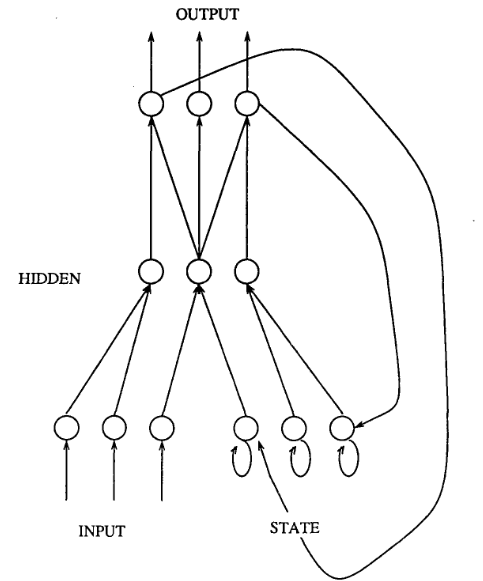
\includegraphics[width=.5\linewidth]{RNNIllustration.png}
        \caption[Schema of a Jordan Network]{Schema of a Jordan Network - \cite{elman1990finding}}
        \label{fig:RNNIllustration}
    \end{center}
\end{figure}

So, when evaluating a sample, the input layer receives not exclusively the values of the independent variables of the sample, but also some values that depend on the previous samples that were evaluated.
The ability to modify the output depending on the previous sample evaluated is what allows it to have some type of memory.
As discussed previously, this is an aspect very desirable for our problem.

Indeed, Xu \textit{et al.} \cite{Xu16} made use of recurrent neural networks to tackle the hard drive failure prediction problem.
Their setup for the neural network is quite standard, up until the point in which they introduce the concept of health status.

So, differently from every other approach in the literature they do not divide the samples in only two classes.
They actually use a more general method in which samples are divided in $N$ classes.

The ones from hard drives that do not fail during the observation period are given the label $N-1$.
The samples from failing disks are divided in the other $N-1$ classes, labeled from $0$ to $N-2$.
The algorithm they use to assign the failing samples divides them depending on how close they are to the failure by using fixed-length intervals.

We can formally define the approach that they explained in natural language in their paper as follows:
suppose that the last $n$ samples from each failing disk are kept in the training set and need to be divided in $N-1$ bins numbered from 0 to $N-2$.
Let the last sample from a specific hard drive before it fails be taken at time $T_i$.
Then, supposing that a sample is taken every 1 unit of time (usually once per hour) the class $c_i(t)$ of the sample of the disk $i$ at time $t$ is given by:

\begin{equation}\label{eq:linear_discrete_health_status}
  c_i(t) = 
  \begin{cases}
    & N-1 \text{, if } i \in \mathbf{healthy} \\
    & \biggl\lfloor(T_i-t)\dfrac{(N-1)}{n}\biggr\rfloor, 0 \leq T_i - t < n \text{, if } i \in \mathbf{failing}
  \end{cases}
\end{equation}

Here, $\lfloor x \rfloor$ is the floor of $x$, meaning the largest integer smaller than or equal to $x$.
For example, $\lfloor 1.8 \rfloor = 1$, $\lfloor 3 \rfloor = 3$.

By analyzing this formula, we see that the $\dfrac{n}{N}$ samples closest to the moment of failure are assigned to class 0, the next $\dfrac{n}{N}$ are assigned to class 1 and so on.

We can also prove that the formula indeed does what is desired, that is, it assigns a number from 0 to $N-2$ to each sample.
In order to do so, we notice that since we have $n$ samples, and the last one is taken at time $T_i$, the first one is taken at $T_i - n + 1$.

We can compute $c_i(T_i) = 0$ and $c_i(T_i - n + 1) = \biggl\lfloor(N-1)\left(1-\dfrac{1}{n}\right)\biggr\rfloor + 1$.
Since $\left(1-\dfrac{1}{n}\right) < 1$, $\biggl\lfloor(N-1)\left(1-\dfrac{1}{n}\right)\biggr\rfloor < N - 2$, so $c_i(T_i - n + 1) \leq N - 2$.
Moreover, $c_i(t)$ is clearly monotonic, since it is a composition of the floor function and elementary mathematical operations.

So, we can guarantee that the formula given above for $c_i(t)$ correctly assigns each sample to a class from $0$ to $N-2$ in which the closer the sample is to the moment the drive fails, the smaller is the value of its class label.

Here it is important to stress that even though both Xu \textit{et al.} \cite{Xu16} and Li \textit{et al.} \cite{Li14} use the term health status, they do not mean exactly the same thing.
The main distinction is that the latter used continuous values in order to train a regression tree, so, there is the idea of a class being closer or far apart from another.

The former, on the other hand, divides the samples in discrete, independent classes.

So, when training the recurrent neural network model, the $N$ classes are completely independent.
Concretely, it does not use the fact that when the correct output for a certain sample is 0, it is better to classify it as belonging to class 1 than to class $N-1$.

Even though the health status is a useful abstraction, there is a need to classify the sequence in itself in only two classes.

In order to do that, when they want to predict the status of a certain drive, they take its last $n$ samples.
Then, from the oldest to the most recent they put each sample as input to the network.
The order in which they are evaluated is important, since the model being used is an RNN and therefore has memory.

For each sample, they classify it as belonging to the class whose associated output neuron value is maximum.
By doing this, it is obtained a sequence of integers $c = (c_1, \dots, c_n), 0 \leq c_i \leq N-1$.

For each $j \in \{0,\dots,N-1\}$, let $C_j$ be the cardinality of $j$ in $c$.
It is clear that $\sum_{j=1}^N C_i = n$.
Then, they define two algorithms, the Voting Algorithm which Tends to Health (VAT2H) and the Voting Algorithm which Tends to Failure (VAT2F):

\begin{equation}\label{eq:vat2h}
    \text{VAT2H}(C) = 
    \begin{cases}
        & \text{Healthy, if } \sum_{j=0}^{N-3}C_j \leq C_N \\
        & \text{Failure, otherwise}
    \end{cases}
\end{equation}

\begin{equation}\label{eq:vat2f}
    \text{VAT2F}(C) = 
    \begin{cases}
        & \text{Healthy, if } \sum_{j=0}^{N-3}C_j < C_N \\
        & \text{Failure, otherwise}
    \end{cases}
\end{equation}

Notice that the contribution of the class $N-2$ is ignored in both algorithms.
This implies that these algorithms only work for when $N \geq 3$.

So, their approach is to extend the problem by expanding the number of classes from 2 to $N$ using equation \ref{eq:linear_discrete_health_status}.
Then, after the network classifies a sequence of samples of the same disk in the classes from 0 to $N-1$ they use equation \ref{eq:vat2h} or \ref{eq:vat2f} to obtain the final binary classification output.

They perform their tests on three different datasets corresponding to different models of hard drives.
The neural network for each model is trained independently since, as discussed, not only the behavior of hard drives of different models can be different \cite{Xu16}.

They obtained promising results with their method.
The FDR of their models was around 97\% while the FAR was almost always kept below 0.1\%.
As was expected, the VAT2H algorithm resulted in a lower FDR and a lower FAR than the VAT2F algorithm.

Nevertheless, their study admitted to having some limitation such as not studying the impact of other health status algorithms different from the one in equation \ref{eq:linear_discrete_health_status}.
Moreover, they used a fixed amount of classes with $N=6$ all over their research.

\section{Long Short-Term Memory}\label{sec:lstm}

Time has proved that RNNs are an effective method to tackle multiple sequence-based problems such as NLP \cite{tarwani2017survey} and video processing \cite{yadav2022survey}.

However, RNNs suffer from a limitation called the vanishing gradient problem.
This limits their efficiency when they need to learn long term dependencies.

This has been proven theoretically by Hochreiter \cite{hochreiter1998vanishing} as well as by Bengio \cite{bengio1993problem} using different approaches.
The intuition behind this result can be explained using the concept of error signal defined in Equation \ref{eq:error_signal}.

If we expand the bottom expression to explicitly write $e_i^{(l)}$ in terms of the error signals of layer $l+2$ instead of $l+1$, we obtain:

\begin{equation}
    e_i^{(l)} = \varphi '(u_i^{(l)}) \sum_j w_{ij}^{(l)} \left(\varphi '(u_j^{(l+1)}) \sum_k w_{jk}^{(l+1)} e_k^{(l+2)}\right)
\end{equation}

From this, we can see that $\dfrac{e_i^{(l)}}{e_i^{(l+2)}} \propto \varphi '(u_i^{(l)})\varphi '(u_j^{l+1})$.
So, it is proportional to the product of two derivatives.
We can extend this process to show that the impact induced by layer $l + m$ on layer $l$ must be scaled by the product of $m$ derivatives.

\begin{figure}
    \begin{center}
        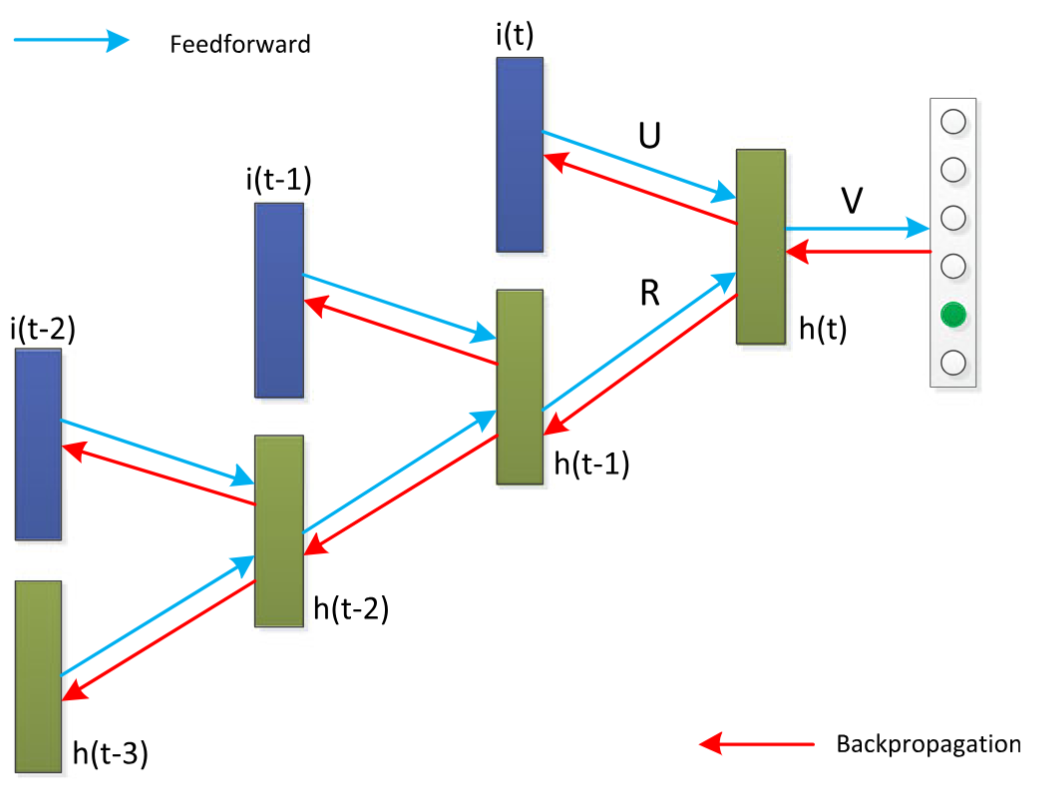
\includegraphics[width=.5\linewidth]{BPTT.png}
        \caption[Backpropagation Through Time]{Backpropagation Through Time interpretation of an RNN - \cite{Xu16}}
        \label{fig:BPTT}
    \end{center}
\end{figure}

But, if we redraw our RNN to be represented as in Figure \ref{fig:BPTT}, we see that the input of sample $t$ can be interpreted as being connected to the output of sample $t'$ by $(t'-t + 1)k$ layers, since it has to traverse the network with $k$ layers $t'-t+1$ times.
So the impact of the sample $t$ on sample $t'$ is proportional to $\prod_{i=1}^{(t'-t)k}\varphi'(x_i)$.

But, if the values of $\varphi'(x_i)$ are all smaller than 1, not only the scaling term will approach 0, but it will do so exponentially fast with respect to the distance between the two samples.

What Bengio showed on his paper \cite{bengio1993problem} is that, as a network learns, these derivatives decrease and become smaller than 1.
From this result, he was able to prove that, as the distance between two samples increase, the impact of the earlier one on the other on the RNN tends to zero.

The only assumption he made was that the model was not sensitive to noisy perturbations.
This is equivalent to stating that if two data sets are similar, then the model is able to learn approximately the same pattern, which is the case of every useful RNN.

So, there is a theoretical demonstration that for long enough sequences, the RNN architecture will be subject to the vanishing gradient problem.
However, theory alone is not enough to define what is a long enough sequence.
In order to state that the vanishing gradient problem has an impact on RNNs it is needed to observe such phenomenon in real-world scenarios. 

And, indeed, experiments show that problems as diverse as sentiment analysis \cite{raza2021cloud} and greenhouse gas predictions \cite{ludwig2019comparison} can be better learned by networks that try to solve the vanishing gradient problem such as LSTMs.

Other research projects show that applying techniques explicitly developed to curb the vanishing gradient problem can result in better results even without needing to change the architecture at all.
For instance, in \cite{hu2021handling} they adapted the activation functions by increasing the value of their derivatives and observed an improvement on the performance of the model.

With this evidence, both theoretical and experimental, it is clear the need to develop networks that are able to better handle or completely avoid the vanishing gradient problem.

So, after proving the vanishing gradient problem in RNNs, Hochreiter developed a network that did not suffer from this problem \cite{hochreiter1997long}.
His solution was the Long Short-Term Memory architecture.
A schematic view of such network is presented on Figure \ref{fig:LSTMSchema}.

\begin{figure}
    \begin{center}
        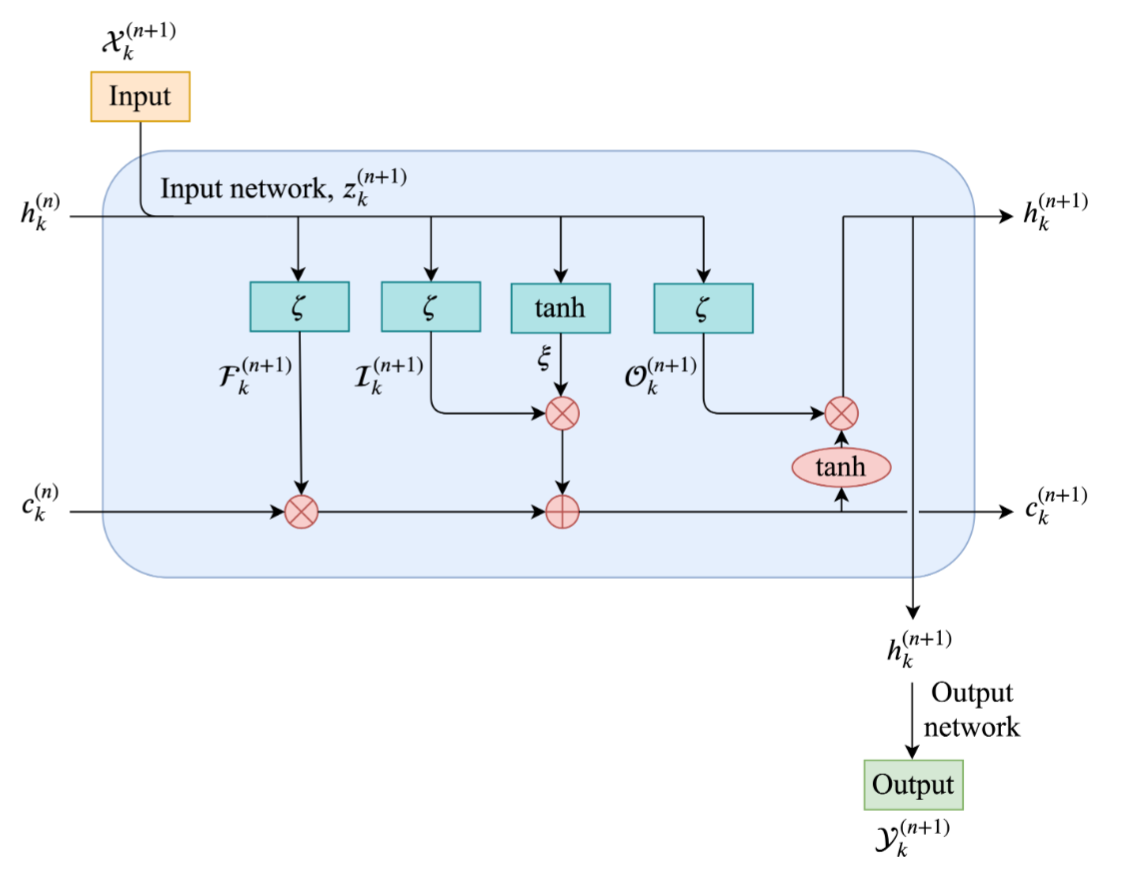
\includegraphics[width=.6\linewidth]{LSTM-Schema.png}
        \caption[Schema of an LSTM]{Schema of an LSTM - \cite{rahman2019nonintrusive}}
        \label{fig:LSTMSchema}
    \end{center}
\end{figure}

Similarly to the RNN architecture, we combine the output of the previous sample (represented by $h^{(n)}$ on the image) with the input data for the current sample ($\chi^{(n+1)}$).
However, the main innovation is the presence of the cell state: the channel represented by the horizontal lane in the bottom half of the image and dented by $c^{(n)}$.

It is not updated using the same logic of the neurons used by BPNNs and RNNs, so it is not subject to the vanishing gradient problem.
The operations performed by an LSTM can be explained in three steps, each one called a gate.

The first one is called the forget-gate and is represented in the image by the leftmost $\zeta$ node.
It takes the input of the current sample ($\chi^{(n+1)}$) and the last output ($h^{(n)}$) of the network and generates a forget-factor vector $P^{(n+1)}$ which is then multiplied component by component with the current value of the state $c^{(n)}$.

The name from this gate comes from the fact that it controls how much the network remembers from the past samples.
In the limit case in which $P^{(n+1)} = \mathbf{0}$, the value of $c$ is reset, and no information is kept from previous iterations.

The next step is the input gate, which in the image corresponds to the central $\zeta$ and $\tanh$ nodes.
If the forget gate decides how much from previous iterations should be kept in the cell state, the input gate controls which data from the current one should be added to the cell state.

The input gate is divided in two steps: the first is to generate the candidate values $\xi$ and the second is to compute the weights $I^{(n+1)}$.
Then each component of the candidate values vector is multiplied by its corresponding weight and added to the cell state.

Finally, there is the output gate that will actually compute the predicted output value for the sample.
In the image it is represented by the rightmost $\zeta$ and $\tanh$ gates.

This is the step that uses the cell state as input.
It combines the cell state value as well as the sample input $\chi^{(n+1)}$ and the previous sample output $h^{(n)}$ to compute a prediction $h^{(n+1)}$ for the current sample. 

In the previous paragraphs, we used generic terms such as compute and generate.
However, for an LSTM, the equations to calculate each term presented above is well-defined and are given by:

\begin{equation}\label{eq:lstm_calculations}
    \begin{cases}
        P^{(n+1)} &= \zeta(W_f\cdot[h^{(n)}, x^{(n+1)}] + b_f) \\
        I^{(n+1)} &= \zeta(W_i\cdot[h^{(n)}, x^{(n+1)}] + b_i) \\
        \xi &= \tanh(W_\xi\cdot[h^{(n)}, x^{(n+1)}] + b_\xi) \\
        C^{(n+1)} &= P^{(n+1)} \odot C^{(n)} + \xi \odot I^{(n+1)} \\
        O^{(n+1)} &= \zeta(W_o\cdot[h^{(n)}, x^{(n+1)}] + b_o) \\
        h^{(n+1)} &= O^{(n+1)} \odot \tanh(C^{n+1})
    \end{cases}
\end{equation}

In the equation above, $[x, y]$ is the concatenation of vectors $x$ and $y$ and $x \odot y$ is the Hadamard or element-wise product.
Also, $W_x$ and $b_x$ represent, respectively, the weights and bias of the network when computing variable $x$.
These are the values that need to be learned during the training process.

When it comes to applying this architecture to solving the hard drive failure prediction problem, there is not much relevant research about using LSTMs that has been published.
Nevertheless, there are some related works.

The first of them was done by Zhang \textit{et al.} \cite{zhang2017deep}.
The main objective of their work was to develop a symbolization-based feature extraction algorithm to improve event detection in LSTMs.

To show the impact of their approach they did perform an experiment on hardware failure detection.
However, they were presenting a more general method.
Consequently, they used different metrics such as balanced accuracy instead of FAR and FDR that would allow us to directly compare with other methods.

Despite us not having access do the desired metrics we can deduce some aspects of their results that allow us to compare to other works.
In order to do that, let positive be the event of the hard drive failing and negative the event of it not failing.

We then introduce the definition of Balanced Accuracy(BA), which was the metric used in \cite{zhang2017deep}:

\begin{equation}\label{eq:ba_def}
    BA \equiv \dfrac{1}{2}\left(\dfrac{TP}{TP + FN} + \dfrac{TN}{TN + FP}\right)
\end{equation}

But this is the average of the recall and the true rate negative, so we can plug the values from Equation \ref{eq:fdr_far} into Equation \ref{eq:ba_def} to obtain:

\begin{equation}
    BA = \dfrac{FDR + (1-FAR)}{2}
\end{equation}

So, even though it is not possible to retrieve the FDR and the FAR by themselves, it is possible to find a range of possible values for them from the balanced accuracy value.

In \cite{zhang2017deep}, the best BA they achieved over all the experiments with the LSTMs, with or without their feature extraction algorithm, was $85.2\%$.
But, since BA is the average of FDR and $(1-FAR)$, it implies that one of these values is at most $85.2\%$, else their average would be bigger.

So, either the FDR they achieved is under $85.2\%$ or their FAR is above $14.8\%$ which is much worse than the one achieved with any other methods we have discussed.

This indicates that their research cannot be used as a reference for the Hard Disk Failure Detection Problem.

There is an additional paper by Das \textit{et al.} \cite{das2018desh} that also applies LSTM to hardware failure detection.
However, it is not for hard drives in data centers, but rather to nodes in a supercomputer which leads to a profile much different from the papers discussed so far.

The first notable difference is that the time scales in which it operates is much smaller.
The TIA they achieve is of the order of 100 seconds, which shows a behavior unlike the one found in data centers in which it is possible to predict a failure more than 100 hours in advance \cite{Li14} \cite{Zhu13}.

But the most important difference is that in \cite{das2018desh} they try to predict failures that happen in components other than the hard drive.
So, they do not make use of SMART attributes, they instead analyze system logs.

Therefore, their motivation to use LSTMs is to detect patterns in text rather than to study time-series.

The FDR they achieve with their LSTM-based approach is between $85.1\%$ and $87.5\%$.
However, it is not possible to compare it to the other results presented above since their problem is quite different from the detection of hard drive failures in data centers.

\section{Additional State of the Art methods}

There are a few additional methods that have been used to tackle the hard drive failure prediction problem and that are worth mentioning.
Since these approaches will not be implemented by our current work, we will limit ourselves to a briefer explanation of the theory behind them.

\subsection{Random Forest}\label{subsec:randomforest}

One of the problems faced by decision trees, specially when they become large is overfitting \cite{ying2019overview}.
This is due to the fact that the split values for each attribute used by the tree are directly taken from the values on the training set.
So, when the tree is deep and there are only a few training samples in a node, the splitting values will sharply follow the ones in the training set.
This is what leads to overfitting \cite{Bramer2020}.

In order to tackle this, Random Forests has been introduced \cite{ho1995random}.
The idea is to train multiple, independent decision trees at once, each one trained with a different subset of the training data.
Notice that these subsets do not have to be disjoint, specially when the training set is relatively small.
This approach reduces the probability of overfitting, since a sample will not be seen by some trees.

Random Forests have performed well for a variety of tasks, ranging from image recognition to Alzheimer's disease detection and prediction \cite{shaik2019brief}.

Research by Shen \textit{et al.} \cite{Shen18} used Random Forests for hard drive failure prediction.
One of the most interesting aspects of their research is how they combined the results of the different trees of the forest in order to evaluate a sample.

Their approach is to not simply feed a sample to every tree in the forest and check which of the two outputs appeared more frequently.
Instead, they gave different weights to the output of each tree based on a clustering algorithm.

More specifically, they performed two independent clustering processes, one for the failing and another to the non-failing samples.
Then, when predicting the outcome for an unseen sample, the clusters $c_0$ and $c_1$ to which it would belong if it were failing or non-failing sample, respectively, are computed.

Since it is known which samples of the training set were used to train each tree, it is possible to evaluate the accuracy of each tree for the training samples in $c_0$ and in $c_1$.
Based on these accuracies, it is possible to give a bigger weight to trees that better learned the samples of the clusters to which the sample being evaluated belongs.

They used a simple algorithm in which the weight of a tree is either $0$ or $1$.
If a tree output a prediction that the current sample being evaluated corresponds to a failing disk, its vote will only be taken into account if its accuracy for samples in $c_0$ that also belong to the training set of the tree is at least $0.5$.
The same will be doing if the prediction of the tree is of a healthy disk, but instead its accuracy will be evaluated over the disks in $c_1$.

Despite this simplicity, they were able to achieve a great performance.
The FDR obtained was above 98\% while the FDR was kept under 0.1\% for multiple scenarios.

What allowed them to get these excellent outcomes, besides of course the algorithm, was their dataset that contained more than 2 million samples of SMART attribute snapshots.

\subsection{Support Vector Machine}

A Support-Vector Machine (SVM) is a non-probabilistic classifier \cite{cortes1995support}.
The idea behind it is to plot the samples in an $n$-dimensional space, in which $n$ corresponds to the number of features in the vector.

Then, the algorithm finds the hyperplane that minimizes its loss function.
The points on one side of the hyperplane correspond to the positive class and the other to the negative class.

The main drawback of SVMs is that drawing a hyperplane means that it can only detect linear dependencies.
So, if there are points in a 2D-plane and the boundaries between the healthy and failing classes is the circumference centered at the origin with radius 1, there is no way that a line can be drawn to correctly divide both regions.

The solution to this is to use the kernel-method, in which dimensions of the original vector are combined using non-linear function and the output of the function is assigned to a new component of the sample vector.
This allows the SVM to correctly learn non-linear dependencies between the variables.

Suppose we want to identify two classes of points that are described by points in a plane.
A class is denoted by the points inside the circle centered at the origin with radius one and the other are all other points.
It is impossible to draw a line in two dimensions that correctly separates both classes.

However, in this example, we can transform the vector $v = (x, y)$ into $v' = (x, y, x^2 + y^2)$ and then and apply the SVM to the set of $v'$.
Then the SVM can potentially learn the plane $z = 1$ (or something similar to it) and thus solve the classification problem without needing to learn explicitly non-linear dependencies.

When it comes to applying SVMs to predicting hard drive failure, the best results were achieved in \cite{Zhu13}.
They used hyperparameters on their model in order to prioritize either a small FAR or a big FDR.

When optimizing for the smallest FAR possible, Zhu \textit{et al.} obtained a FAR of $0.03\%$ and an FDR of $68.5\%$.
When priority was giving to increasing the FDR, they obtained a FAR of $0.3\%$, but the FDR was increased to $80.0\%$.

Support-Vector Machines, when compared to other approaches, present, therefore, a method that is able to achieve a smaller FAR.
However, in contrast, it is not able to attain FDRs as good as other methods while keeping an acceptable FAR.

\subsection{Linear Regression}

An approach using one of the simplest statistical learning methods, linear regression, has been proposed for the hard drive failure prediction problem.
Yang \textit{et al.} \cite{yang2015hard} showed described a methodology to obtain good results with a linear regression model.

In order to allow a simple method to detect rather complex relationships as the ones that can occur between the value of SMART attributes, the focus of their work was on feature engineering.
More specifically, they started by dividing values of each SMART attribute in different bins.
Then, depending on the bins occupied by the attributes of a hard drive, the SMART values were translated in a set of features.

Since some specific combinations of bins were required for the algorithm to assign a certain feature to a hard drive, the feature space was sparse.
This means that a single disk did not satisfy the conditions to be assigned most of the features.

The main drawback of this approach is the need for massive amounts of data.
In their work they state that their dataset, consisting of more than 7 million samples, contains 500 times more samples of SMART attributes than any other work on this problem.
Not only this data may be not trivial to obtain, but also it is accompanied by a necessity of a substantial computing infrastructure to process it.

An important aspect of their approach is that no distinction was made between hard drives whose models were different.
This is a sharp contrast with other research on the subject that explicitly train different machine learning models for different disk models \cite{Xu16} \cite{Shen18} \cite{Li14}. 

Despite this limitation, their results were promising, showing an FDR of 97.8\% with an FAR of 0.3\%.
However, they also showed that the huge amount of data they used to train their model is a non-negotiable requirement.
For a subset that only included 1/512 of the original dataset samples, meaning that its size was comparable to the one in other works, even for an FDR of 0.5\%, the FDR is below 40\%, which is much worse than other work done on the same problem.

\subsection{Convolutional Neural Networks}

A Convolutional Neural Network (CNN) is a machine learning model.
It is usually applied to computer vision tasks.
Just like BPNNs discussed in Section \ref{sec:BackpropagationNeuralNetwork}, it is not recurrent meaning that the output for a certain sample is not propagated to following ones.

The main aspect that differs a CNN from a BPNN is the presence of convolutional layers \cite{o2015introduction}.
In a convolutional layer, a neuron in layer $l$ is not connected to every neuron in layer $l-1$.
Instead, it is connected to a few consecutive nodes of layer $l-1$.

This is useful for handling data that is represented as a vector with many components, such as images, in which each pixel corresponds to an input.
For a 100x100 image, fully connecting two layers would require 10,000 weights.
By using a 5x5 convolution window with shared weights, it is possible to reduce this value to only 25 weights, or 400 times less.
This allows the network to be much deeper.
 
A relevant attribute of a CNN is its translation invariance \cite{kayhan2020translation}.
The use of shared weights implies that shifting some values by a certain constant value does not hinder the network's ability to recognize a certain pattern.
This is because the convolutions will be performed with the same weights no matter in which part of the image a certain sequence of values is.

It was exactly this translation invariance aspect of the CNN that motivated Sun \textit{et al.} \cite{sun2019system} to adapt CNNs to handle time series to tackle the hard drive failure prediction problem.
For a time-series, translation invariance implies that a pattern due to a sequence of values or events can be detected independently of where in the sequence it occurs.

In order to obtain, they also had to adapt the loss function to handle the imbalanced dataset that contained many more healthy samples than failing ones, which is an intrinsic aspect of the problem at hand.

So, they gave a bigger weight to samples from failing disks that were misclassified, else the model would be prone to classify almost every disk as a healthy one.
This is due to the fact that, with a classic loss function, even if the model misclassified every failing disk, its total loss would be much smaller than if it misclassified even a small percentage of the healthy disks.

In their results, the metric they presented that we can use to compare with other methods was the recall, which corresponds to the FDR.
They achieved an FDR of $65\%$ which is considerably smaller than the one attained by other models.
But this is partly due to the fact that they used a heterogeneous dataset, meaning that they did not train different networks for different hard drive models.
\chapter{Methods}\label{chap:methods}

The objective of this thesis is to compare different approaches to tackle the hard drive failure prediction problem using SMART attributes.
However, we do not limit ourselves to already published results, and we implement a program capable of executing the training and evaluation processes for different models.

This allows us to not only to more objectively compare the different methods by running them on the same dataset, but also to more deeply explore the influence of some steps of the pipeline such as the feature selection and the voting algorithm on the performance of the models.

Finally, the current work aims to more thoroughly test the impact of the health status approach proposed in \cite{Xu16}.
This can be done by using it to train other models to measure how much of the results of \cite{Xu16} is due to the use of an RNN and how much can be attributed to the concept of health status.
Since this is not a method commonly used in literature, it requires us to implement it ourselves.

\section{Health Status}\label{sec:health_status}

The current work aims to apply the concept of health status introduced in \cite{Xu16} and \cite{Li14}.
We intend to find how powerful this concept can be to improve the performance of different types of models.

The idea is to not map all healthy samples to a class labeled 1 and all failing samples to a class labeled 0.
Instead, we can extend the range of different labels beyond these two values.

The rationale behind it is that samples of a failing disk that were taken closer to the moment of failure probably better describe a failing disk than the ones from the same disk that were taken much before the critical moment.

However, some samples not taken as close to the moment of failure can still provide some useful data, so we try an approach that treats this data differently instead of simply removing and ignoring it.

Now, the challenge is to determine how to map different samples of the same disk to distinct values.
Let $n$ be the number of samples from a failing disk that we consider as belonging to the critical window.

The first health status algorithm we have is the one we will call the Discrete Health Status Algorithm.
It is the one used by Xu \textit{et al.} \cite{Xu16} and is described by Equation \ref{eq:linear_discrete_health_status}.

One of the main advantages of using it is that if we set $N = 2$ in Equation \ref{eq:linear_discrete_health_status}, we will get label $0$ for the failing disks and $1$ for the healthy ones.
So, we can consider this method a generalization of the \textit{ad-hoc} labeling that is used in most binary classification problems and that can applied for any time-series based problem.

The second approach we can use for an algorithm that computes the health status of a certain sample is to drop the constraint that it must be an integer, while still keeping it linear and mapping every value to the interval $[0,N-1]$.

So, we propose the following algorithm that we will refer as the Continuous Health Status Algorithm:

\begin{equation}\label{eq:continuous_health_status}
  c_i(t) = 
  \begin{cases}
    & N - 1 \text{, if } i \in \mathbf{healthy} \\
    & (T_i-t)\dfrac{(N-1)}{n}, 0 \leq T_i - t < n, \text{, if } i \in \mathbf{failing}
  \end{cases}
\end{equation}

The continuous health status algorithm completely abandons the concept of classes and instead uses a score system.
It is particularly useful for the regression tree model because it does not need any modification in order to handle real values.
On the other hand, the other methods require the training data to be divided in discrete classes.

\section{Models}\label{sec:models}

In total, we have implemented five distinct models to tackle the hard drive failure prediction problem.
Namely, they are classification tree, regression tree, BPNN, RNN and LSTM.

The theory behind the models we implemented was explained in Chapter \ref{chap:background}. 
So, in the following section, we present how each of them was implemented to tackle the hard drive failure detection problem, both using the classic approach and using the health status technique.

The discussion in this section concerns how to train each model to predict the class of individual samples.
Later on, on Subsection \ref{subsec:voting}, we will show the process we apply to use the output of a model corresponding to a hard drive's sample in order to obtain a verdict for the disk. 

\subsection{Decision Tree}\label{subsec:decision_tree}

Classification and regression trees can be grouped under the umbrella term decision tree.
Despite this, their application to the problem at hand is not done the same way.

Classification Tree is a model designed to tackle classification problems as its name suggests.
Therefore, once we are trying to determine if a hard drive is going to fail soon or not, and we have a set of SMART attributes, the idea to try this model follows trivially.

However, the main drawback of a classification tree is that it cannot easily assign a degree of confidence to its result, since it is limited to outputting an integer corresponding to a class.

The regression tree allows us to tackle this limitation by not looking at the problem from a classification point of view.
Instead, it aims to assign a score to each sample, which can be a real number.

For the regression tree, the concept of classes does not even exist.
It is up to us to map the classes to scores that are fed to the model and then interpret its output to map it to a class of our problem.

So, it can be an extremely powerful tool as long as we can assign scores instead of labels to our samples.
Therefore, the approach of using the continuous health status matches perfectly with this use case.

In order to train a classification tree and a regression tree, the training set is formatted the same way: a set of samples of SMART attribute values labeled with their corresponding health status.
The only limitation is that the classification tree is limited to integer values of health status.

On the other hand, the output produced by both models is quite different.
When an unseen sample is given to the classification tree, it will simply output an integer value between $0$ and $N-1$ corresponding to the predicted class.
In contrast, the regression tree can produce a score which is a real number.

\subsection{Neural Networks}\label{subsec:nn}

We use three different neural network architectures: BPNN, RNN and LSTM.

The idea behind using a BPNN is similar to the one to use decision trees: it can work well for problems in which we have to classify samples based on real valued feature vectors.

On the other hand, RNNs and LSTMs work quite differently.
As discussed in sections \ref{sec:RecurrentNeuralNetwork} and \ref{sec:lstm}, these networks are adapted to handle sequences of values instead of processing different samples independently.
This lends itself perfectly to our use case in which we have in our dataset different time series. 

This difference allows us to divide our models into two different groups.
We will call one the time insensitive class and the other the time sensitive class. 

Time insensitive models are the ones that treats each sample independently even though some come from the same hard drive.
So, these are the ones that do not have a direct way to model time dependencies.
In our experiments, these are classification and regression tree and BPNN.

In contrast, time sensitive models expect to receive a sequence of samples of the same hard drive in chronological order, since they are able to model how the values of a sample at a previous time impact the current one.
These are RNN and LSTM in our experiments.

The input data expected by the BPNN is therefore similar to the one for decision trees discussed in Subsection \ref{subsec:decision_tree}: a set of samples and health status values that are independent.
This is the case for both the training and testing processes.

The time sensitive models, however, add some additional constraints to the input data.
The samples from the same disk must be fed in chronological order in order for them to be able to perform their time propagation operations correctly.
Moreover, the network needs to know where the data from a hard disk ends and data from a new one begins, so it can erase its memory.

Even though all data from a disk is fed sequentially, it is important to notice that the time sensitive models will also generate a different output for each sample instead of classifying the entire sequence at once.

When it comes to the output, we can adapt the architecture of any one of the network-based model to have either one or multiple output nodes.
The former is the classic approach to a binary classification problem in which the output is a value between $[0, 1]$ corresponding to the probability, according to the model, that the given sample belongs to the class labeled as 1.
In practice, this is done by using the logistic function as the activation function of the output layer.

As a consequence of their architecture these models with one output node, can only handle cases in which $N = 2$, so from here on out we will call them binary neural network models.

The second way to organize the output of the neural network is to use a different output node for each of the $N$ classes being predicted.
This time, the constraint of $N=2$ can be dropped.
Because of this, we call the models following this architecture multiclass neural networks.

Each of the $N$ output nodes produces a value that is interpreted as a score assigned to each class.
The bigger the value of the $i^{th}$ output node, the higher the confidence of the model that the sample belongs to the class $i$.

In order to train these multiclass models, we use the one-hot encoding method, in which the vector corresponding to a sample whose health status is $h$ has all its components equal to 0 except for the $h^{th}$ one, assuming 0-based indexing.
So, if $N = 4$ and $h = 1$, the corresponding vector is $(0,1,0,0)$.

\section{Setup}\label{sec:setup}

In this section we describe the components of the experiment beyond the model such as the feature selection and voting algorithms.
We can make these steps of the pipeline identical for different models which allows us to compare them.

\subsection{Change Rate}\label{subsec:change_rate}

The first step is to compute the change rate of the attributes for each sample.
This is done so that models such as decision trees and BPNNs can take into account the fact that we are working with a sequence.

More formally, we choose a positive integer $\Delta t$ that is the same for every sample.
Then for the hard drive $i$ we will have a sequence $(x_{i,t}), t \in \{1,\dots,T\}$ where $x_{i,t}$ is a vector with the SMART values for the disk at time $t$.
We then compute the sequence:

\begin{equation}\label{eq:change_rate}
(x'_{i,t}), t > \Delta t, \text{with } x'_{i,t} = [x_{i,t}, (x_{i,t} - x_{i,t-\Delta t})]
\end{equation}

It is this sequence $(x'_{i,t})$ that is then passed to the next steps of the experiment.

Notice that the first $\Delta t$ samples need to be discarded, since the change rate is not well-defined for them.
This fact, as well as the observation that two samples too far apart should not be as strongly correlated than two closer ones suggest that the value of $\Delta t$ in practice should be kept small.
As a result, for most experiments, we keep $\Delta t$ equal to 1.

This step is completely optional, and the next steps continue behaving correctly if the change rates are not inserted, they just works with smaller vectors.
This allows us to do experiments without the change rate computation to observe its impact on the performance of the models.

\subsection{Feature Selection}\label{subsec:feature_selection}

The next stage of the preprocessing procedure is to perform the feature selection.
Once we have multiple sequences of vectors, we need to decide which features are actually going to be fed to the model.

The feature selection process has become a key step in real-world scenarios in order to remove irrelevant features and reduce the dimensionality of the data.
Models working with more relevant features can more easily learn the problem at hand since a smaller number of relationships between the different attributes need to be found \cite{kumar2014feature}.

For the failure prediction problem we have, the challenge is to remove the features that behave similarly in the healthy and failing disks.
In order to do that we compare 3 different methods: z-score, reverse arrangement and rank-sum.

The three of them compare the distribution of the same feature on the healthy and failing disks.
A feature can be either a SMART attribute or the change rate of a SMART attribute computed in the previous step, but all features are evaluated independently and in the same manner.
If these distributions are very different, the score assigned to the feature is higher than if the distributions are more similar.

The approach used in our experiments is to decide a number $F$ of features to keep.
Then, the $F$ features with the highest score are kept, and the others are discarded.

This is a less biased approach than using a threshold value for the score of a feature in order for it to be kept.
This is due to the fact that these thresholds would need to be different for each feature selection method used since the score distribution depends on the function.
Moreover, this allows for the approach to be more easily generalized for different datasets that can present different behaviors.

The main drawback of this approach is that multiple experiments need to be performed in order to find the value of $F$ that maximizes the performance.

The z-score compares the difference of the means of an attribute over the two classes \cite{Murray2005}.
It is defined as follows:

\begin{equation}
  z \equiv \dfrac{m_f - m_h}{\sqrt{\dfrac{\sigma_f^2}{n_f} + \dfrac{\sigma_h^2}{n_h}}}
\end{equation}

Where $m_f$, $\sigma_f$ and $n_f$ are, respectively, the average of the feature over the failed samples, its standard deviation and the number of failed samples respectively. 
The values $m_h$, $\sigma_h$ and $n_h$ represent the same quantities but for the healthy samples.

If the average of the feature in both classes are relatively small when compared to their variances, then the probability that they come from the same distribution is bigger and the value of $z$ will be closer to 0.

Since for the feature selection step we are interested only on whether they are similar or not and not which the distribution is bigger, we use $|z|$ as the score that the feature selection algorithm actually outputs.

The reverse arrangement test indicates whether a given sequence has a tendency to increase, decrease or to remain constant \cite{Murray2005}.
Let $(f_{i,t}), t \in \{1,\dots,T\}$ be the sequence representing the values of a certain feature for disk $i$.
Then, we define the test statistic $A$ as:

\begin{equation}\label{eq:reverse_arrangement}
  A \equiv \sum A_t, \text{with } A_t \equiv \sum_{j=t+1}^{T} I(f_{i, t} > f_{i, j})
\end{equation}

Here, $I$ is the identity function and is equal to 1 if the condition passed as argument is true and 0 otherwise.

Under the hypothesis that the values of $f_{i,t}$ come from the same distribution that does not change as time passes, then there is no temporal tendency and the expected value of $A$ can be computed as well as its standard deviation.

By analyzing the above formula we notice that if $f_{i,t}$ tends to decrease as times passes, the value of $A$ will be large.
On the other hand, if its tendency is to increase, then $A$ will be small.

So, if the value of $A$ is too far away from the average that can be computed when assuming no time-dependence, it allows us to affirm, up to some degree of confidence, that there actually is a time-dependency of $f_{i,t}$.

For a given value of $T$ and a certain degree of confidence, the lower and upper bounds of $A$ for a time-independent distribution can be computed.
These values are available in tables such as Appendix A.6 of \cite{bendat2011random}.

In our experiment, for each disk we keep its 100 last samples (the disks that fail before 100 samples are recorded are discarded).
Then we compute the value of $A$ for each disk.
We then count the number of failing and non-failing disks in which a time-dependency can be observed with a high degree of confidence.

In order to do this we take into account the upper and lower bounds of Appendix A.6 of \cite{bendat2011random} with $\alpha = 2\%$ meaning that in order for a feature of a disk to be flagged as time dependent there is a probability 98\% that a time-independent distribution would not yield a value of $A$ so far from the expected value.

Finally, the score assigned to a feature is the absolute value of the difference between the number of failing and healthy disks that had this feature flagged as time dependent.
In mathematical notation, for a given feature $f$:

\begin{equation}
  ra(f) \equiv \left| \sum_{d \in \mathbf{failing}} I(A(d, f) > U \lor A(d, f) < L) - \sum_{d \in \mathbf{healthy}} I(A(d, f) > U \lor A(d, f) < L) \right|
\end{equation}

Where $A(d, f)$ denotes the test static defined in Equation \ref{eq:reverse_arrangement} for disk $d$ and feature $f$.
$U$ and $L$ are, respectively, the upper bound and the lower bound of the test statistic for the confidence value we are using.

Taking the difference between the two classes allows handling features that are trivially always increasing or decreasing on both sets.
For example, if we only computed $A$ for the failing samples, some features such as the number of hours the disk is in power on state would always have a high score since it is monotonically increasing for every sample.

The third feature selection algorithm we have used is the rank-sum test, also known as the Mann-Whitney U test.
It works similarly to the other methods by trying to gauge the probability that two sequences of values come from the same distribution.

In order to explain the idea behind this method we take a generic example in which we have two sequences $X = (x_1,\dots,x_n)$ and $Y = (y_1,\dots,y_m)$.
The challenge is to determine with which degree of confidence we can affirm that $X$ and $Y$ were obtained by sampling the same distribution.

The rank-sum test achieves this by first merging the two sequences into a new sequence $Z$ and sorting it.
It uses the fact that if $X$ and $Y$ come from the same distribution, then the values of $X$ will probably be well distributed on the sorted sequence $Z$ instead of being concentrated at the beginning or at the end.

So, let the elements of $X$ be at positions $(p_1, \dots, p_n)$ in $Z$ and the ones of $Y$ be at positions $(q_1, \dots, p_m)$.
We notice that $(p_1, \dots, p_n) \oplus (q_1, \dots, q_m)$ is a permutation of $(1,\dots,n+m)$.
Here $\oplus$ denotes the concatenation of two sequences.
Then, the test statistic $U$ is given by \cite{macfarland2016mann}:

\begin{equation}
  U = \min\left(nm + \dfrac{n(n+1)}{2} - R_1, nm + \dfrac{m(m+1)}{2} - R_2\right)
\end{equation}

With:

\begin{equation}
  \begin{cases}
    R_1 &= \sum_{i=1}^{n}p_i \\
    R_2 &= \sum_{i=1}^{m}q_i
  \end{cases}
\end{equation}

From the values of $U, n, m$ it is possible then to calculate the p-value of the distribution.
The p-value corresponds to the degree of confidence that the hypothesis that both sequences come from the same distribution is true.

So, if, for a certain feature, the p-value obtained is small, we want to keep it since its value is much different on the healthy and failing samples.
Therefore, the score returned by our algorithm is the opposite of the p-value.

\subsection{Train-Test Split}\label{subsec:train_test_split}

In order to correctly train and evaluate our models, we need to split our data into training and testing sets.

This is a delicate process due to the fact that the data is not balanced, meaning that we have many more healthy than failing hard drives, which is a characteristic of the hard drive failure prediction problem.
Also, we deal with distinct models that process data differently and therefore introduce the need for different operations to be performed at this step depending on the model at hand.

As discussed previously, time sensitive and time insensitive models expect the training and test data to be organized differently.

The first step is to do a $70/30$ split of the failing disks.
Since we have a limited amount of failing hard drives, we want to use all of them.
So, we assign $70\%$ of them to the training set and the other $30\%$ to the testing set.

Then, we choose a value $n$ of samples of the failing hard drives in the training set that we will consider as being in the critical window.
This means that we only consider the last $n$ samples before failure as describing a failing hard drive.

As we have discussed in Section \ref{sec:health_status} not all of these $n$ samples are treated equally, our experiment takes into account how close to the failure point each sample is.
However, at this point we can already discard every sample from a failing disk in the training set that is not one of the last $n$ taken for the corresponding hard drive.

Also, we need to choose a healthy-failing ratio $r$ meaning that for each sample from a failing disk in the training set, we will have $r$ from healthy hard drives in it.

For the time insensitive models, we simply split the healthy disks in training and test sets using a $70/30$ split.
Then, if the training set has $f$ failing disks, each contributing with $n$ samples, then we choose at random $b\cdot n \cdot r$ samples from the healthy training set to include in the final training set.

The other $30\%$ of the healthy and failing disks form our test set.
The split of the disks is necessary before the sampling in order to ensure that disks in the testing set have not been seen by the model while training it.

Also, it is important to notice that no sample from a disk in the test set is discarded.
This allows the evaluation to be performed in a real world like scenario in which no information about the future of the disk is known. 

For the time sensitive models, the sampling step of the healthy disks to include in the training set is a little more delicate.
This is due to the fact that we need to obtain sequences coming from the same disk to train the models, so the sampling process cannot choose samples independently.

So, we use the fact that, for every disk that did not fail during the observation period, the same number $m$ of samples have been measured for each of them.

Therefore, to form the training set, we choose $\dfrac{b\cdot n \cdot r}{m}$ distinct hard drives and include all of their samples.
In the end, we will have $\dfrac{b\cdot n \cdot r}{m} \cdot m = b\cdot n \cdot r$ samples from healthy disks.
This is the same number that we have for the time insensitive models, just organized differently.

This allows us to directly compare the results for different values of $n$ and $r$ without depending on other characteristics of the dataset.

\subsection{Health Status}\label{subsec:health_status}

Before training our models, we need to perform a last preprocessing step that corresponds to computing the health status value corresponding to each hard drive sample.

We then can use either the continuous or discrete health status algorithms described in Section \ref{sec:health_status}.

The multiclass neural networks and the classification tree models only support the discrete version of the algorithm.
This is due to the fact that they work directly with the idea of classes.

The binary neural network models also have been designed to handle the discrete health status algorithm.
However, they have the additional constraint of $N = 2$.

The regression tree can make use of both algorithms.

\subsection{Training}

After performing the train-test split and computing the health status for the training samples, we can feed the training set to our models in order to train them.
The specifics of the differences between each model have been presented in Section \ref{sec:models}.

\subsection{Voting}\label{subsec:voting}

The final step is to actually apply the models to the samples on the test set.
This allows us to evaluate if the model has learned to predict hard drives failures for samples it has not yet seem.

In a real world scenario we will have, for each disk, a sequence $(x_1,\dots,x_n)$ of its SMART attribute values taken at nearly constant intervals.
The objective is to determine if these samples allows us to say that the disk is going to fail in the near future.

At this point, we assume that we have a model that is able to take a sample (or a sequence of them in the case of time sensitive models) and generate a prediction for it.
The format of this output can be slightly different depending on the model's architecture.

The \textit{ad-hoc} approach is to only consider the output of the model for the sample $x_n$.
If it corresponds to a failing sample, we flag the disk as going to fail soon.

However, a more robust approach is to take into account an interval of $v$ consecutive values $(x_{n-v+1},\dots,x_n)$.
Imagine the case in which there is a single sample classified as failing surrounded by tens of others that the model predict as healthy.
Then, probably, the hard drive is still working as intended.

In order to make the final decision of whether a disk is going to fail or not, we choose two values: the number of votes $v$ and the voting threshold $\tau$, which is a number between 0 and 1.
Then we give the samples $(x_{n-v+1},\dots,x_n)$ to our model and receive the outputs $(y_{n-v+1},\dots,y_n)$.

For the time sensitive models, we pass the values $(x_{n-v+1},\dots,x_n)$ as a sequence instead of evaluating them independently and resetting the memory of the model after seeing each sample.
This is the method we have devised to take advantage of their capability to process sequences that yield the best results.

We then propose to combine the values of the outputs two different ways in order to obtain the final prediction of the model.
The first we will call Class Based Voting algorithm and is inspired by \cite{Xu16}.

We first convert each $y_i$ into a class $C_i$.
This is done differently according to the model at hand.
For a classification tree, it is straightforward: $C_i = y_i$, since the output is already an integer.

For a regression tree, we do $C_i = \min(\max(0, \lfloor y_i \rceil), N-1)$.
Where $\lfloor z \rceil$ denotes the closest integer to $z$.
The min and max functions allows us to handle cases in which $y_i < 0$ or $y_i > N-1$.

For a binary neural network, we have a similar expression: $C_i = \lfloor y_i \rceil$, since $y_i$ is constrained between 0 and 1.

For a multiclass neural network, we use the class with the largest score in the output vector.
Mathematically, $C_i = \argmax_{j\in\{0,\dots,N-1\}}(y_i[j])$.

Once $C_i$ is defined for each sample, we can obtain a histogram $H$ with the number of samples classified in each class.
Let $H_i$ be the number of elements in class $i$ in the histogram.
We can then use $H$ to determine if the disk is in a healthy or failing state as follows:

\begin{equation}\label{eq:class_based_voting}
    \text{CB}(H) = 
    \begin{cases}
        &\text{Healthy, if } (1-\tau)\sum_{j=0}^{\max(0,N-3)}H_j \leq \tau H_{N-1} \\
        & \text{Failing, otherwise} 
  \end{cases}
\end{equation}

This is similar to Equations \ref{eq:vat2h}.
However, we adapt it to be able to handle the case of $N$ = 2.
Also, it can be seen as a generalization of the voting algorithm in \cite{Li14}, since we introduce the value $\tau$ to be able to change the threshold.

The hyperparameter $\tau$ we introduce here is the voting threshold.
This denotes that a ratio strictly bigger than $\tau$ of the samples being considered (meaning those with $C_i \neq N-2$) have to be in classes other than $N-1$ for the disk to be considered as failing.

It is similar to the Class Based Voting, but with a modified value of $C_i$.

We also propose a second voting algorithm that delays the rounding step done to assign each sample to a class.
We make use of the fact that we get a vector with $N$ scores that can be interpreted as the degree of confidence of the model that the sample belongs to each of the $N$ classes.

When we increase the value of $N$, the number of samples of each class from $0$ to $N-2$ seen during the training decreases, even though the sum over all of these classes remains constant.
So, the model may be more biased towards the class $N-1$ since it has seen more samples with it.

In order to reduce the impact of this bias, we propose a method that recombines the values in classes from $0$ to $N-2$.
The first step is to use the softmax function, denoted by $\sigma$, to convert the values of $y_i[j]$, corresponding to the score the model assigns to the sample $i$ belongs to class $j$, to a probability $p_i[j]$.

\begin{equation}
  p_i[j] = \sigma(y_i)[j] = \dfrac{e^{y_i[j]}}{\sum_{k=0}^{N-1}e^{y_i[k]}}
\end{equation}

Notice that this is a non-linear function and therefore the result of the class given by equation \ref{eq:modified_class} will be affected by it.
Moreover, the values of $p_i[j]$ can be interpreted as a probability that the sample $i$ belongs to class $j$ since the property $\sum_{k=0}^{N-1}p_i[k] = 1$ is verified. 
Then we can use this values to obtain a binary class from the probability of each one of the multiple classes as follows:

\begin{equation}\label{eq:modified_class}
  C_i = 
  \begin{cases}
    & 0, \text{ if } \sum_{j=0}^{\max(0,N-3)} y_i[j] > y_i[N-1] \\
    & 1, \text{ otherwise}
  \end{cases}
\end{equation}

We then make a histogram as before, but with only two bins.
Finally, we apply the following formula that we will call the Score Based Voting Algorithm:

\begin{equation}\label{eq:score_based_voting}
  \text{SB}(H) = 
    \begin{cases}
        & \text{Healthy, if} (1-\tau)H_0 \leq \tau H_1 \\
        & \text{Failure, otherwise} 
  \end{cases}
\end{equation}

For a regression tree, we can still take into account the exact score instead of the class it maps to.
However since the output is a single number instead of a vector of numbers, the formula has to be modified.
We use the following expression, where $y$ is the vector of predictions of the model to the sequence of samples using in the voting process:

\begin{equation}\label{eq:score_based_voting_regression}
  \text{SB}(y) = 
    \begin{cases}
        & \text{Healthy, if} \sum_{i=1}^v y_i \geq v(N-2) \\
        & \text{Failing, otherwise} 
  \end{cases}
\end{equation}

The values of the regression tree are in the interval $[0,N-1]$, with the failing samples in the training set corresponding to values in $[0,N-1]$.
If its average is on $[N-2,N-1]$ the result of the voting algorithm is that the disk is healthy, otherwise it signals the disk as failing.

\subsection{Evaluation}

In order to evaluate the model, we use the test set we described in subsection \ref{subsec:train_test_split}.
It has a series of distinct disks with the expected classification result for each of them: healthy or failing.

In order to simulate what happens in a real-world scenario, for a disk with samples $(x_1,\dots,x_n)$, for each $i \geq v$, we take a slice $(x_{i-v+1}, \dots, x_i)$ of the samples.
We then perform the evaluation and voting processes described in subsection \ref{subsec:voting} using our previously trained model.

If for a value of $i$ we get a diagnosis of a healthy disk, then we continue the process for $i+1$.
If we get to $i > n$ then the verdict of our experiment is that the disk is healthy.

In the case in which the expected diagnosis for this disk was to be healthy, then we add 1 to our count of true negatives.
Otherwise, we add 1 to the number of false negatives.

If for some value of $i$ the voting algorithm indicates that the disk is failing, then the verdict for this disk is that it is a failing one.

If the expected diagnosis for this disk was to be healthy, then we add 1 to our count of false positives.
Otherwise, we add 1 to the number of true positives and store the time in advance with which the failure was detected, that is we store the value of $n-i$.

In the end, this experiments allows us to easily compute the FAR and the FDR for our testing set.
We also compute the average time in advance as well as its standard deviation.

The average TIA indicates how much time, on average, there is to back up the data on the disk and replace it after our system flags a disk as going to fail in order to prevent data loss and disruption of service. 

The standard deviation of the TIA is a measure of how much its value varies from one disk to another.
Ideally, this value should be small to indicate that almost all failures are detected with approximately the same TIA.

\section{Software}\label{sec:software}

In order to perform our experiments and objectively compare the different models, we have developed a program capable of training and evaluating any of the models described above.
To allow others to use our models and eventually extend it, we have made the code open source\footnote{Code available at \url{https://github.com/Miguel0312/health-status-experiment}.}.

We already had in mind the need to test multiple methods for different steps of the experiment, from the feature selection algorithm to the models and the voting algorithm.
So, from the start, the architecture of the program was planned so that it would be highly extensible.

This should make developing new methods and testing them with our library straightforward.
There is also the added benefit that it allows the comparison of the results on the same datasets with different state of the art methods.

The models we used were the implementations from PyTorch (for the neural networks) and scikit-learn (for the decision trees).

We also used an approach of decoupling the declaration of a model from the methods used to train and evaluate it.
Since our models can be split into time sensitive and time insensitive as well as binary or multiclass, for example, different models have different parts of the pipeline in common.

So, a class representing a model declares its network as well as a description, which is a series of flags indicating its attributes such as if it is time sensitive or not, for example.
We then use a dynamic dispatching approach in which a method will read the description of the model and then call the appropriate algorithm.

This can be more concretely observed on the \verb|train_model| method of the \\ \verb|FailureDetectionNN| class.
Instead of overriding this method for each class, it simply calls \verb|utils.trainNN| which will read the values of the description flags and call the correct method.

This makes the code a lot more robust by not repeating code and making sure that a bug that is solved or a modification that is made for one model is propagated to all of them.

We also made the decision of using, for example, two distinct flags \verb|BINARY| and \\ \verb|MULTICLASS| instead of checking for the presence or not of the \verb|BINARY| flag.
This allows future models that are neither binary nor multiclass without making it necessary to modify previously existing code.

Finally, one of the most important features of such kind of library is the ability to train multiple models and modify their hyperparameters without touching the source code.
Therefore, the configurations to the experiments of our library is not done through code but instead through human-readable text files.

Our code is able to read a file and instantiate all the steps needed to train and evaluate using the given hyperparameters.

The file format we chose was TOML (Tom's Obvious Minimal Language).
This language allows us to separate the attributes into different tables such as dataset, preprocessing, model and vote which makes it easier to read, interpret and modify.

Moreover, TOML supports arrays out of the gate.
We used this feature to be able to instantiate multiple experiments from a single configuration file.

Suppose that a field of the configuration file is an array instead of an integer or a string.
Then our code will extend the other fields to also be an array.
For those that are single values such as strings and numbers instead of arrays, it suffices to create a list with multiple copies of the same elements.

This make it much easier to perform multiple experiments at once and, more importantly, to analyze the impact of each of the hyperparameters on the performance of the model.

The configuration files used in our experiments are available in our repository under the name \verb|standard-MODEL-LEVEL| where \verb|MODEL| is the name of the model and \\ \verb|LEVEL| denotes whether the model is binary or multiclass.
When discussing our experiments, any modification of the hyperparameters from the standard files is explicitly mentioned.

\section{Hyperparameters}

In this section we describe the hyperparameters that we were able to control during our experiments.
Most of them correspond to some values that have been introduced on previous sections, but a common vocabulary will be useful later on to discuss the results.
Moreover, it allows the interpretation of the configuration files we make available in our repository.

\begin{itemize}
  \item \textbf{Number of Failing Samples}: the number of failing samples that we consider as belonging to the critical window of a failing disk. 
  It is the value of $n$ on Equations \ref{eq:linear_discrete_health_status} and \ref{eq:continuous_health_status}.

  \item \textbf{Change Rate Interval}: the delta we use to compute the change rates.
  It corresponds to the value of $\Delta t$ on Equation \ref{eq:change_rate}.

  \item \textbf{Feature Count}: the number of features (may it be SMART values or its change rates) to be kept by the selection feature algorithm.
  It is the value $F$ discussed in subsection \ref{subsec:feature_selection}.

  \item \textbf{Feature Selection Algorithm}: the algorithm used to rank the features in order to decide which ones to keep and which to discard.
  There are 3 of them: z-score, rank-sum and reverse arrangement.

  \item \textbf{Health Status Algorithm}: how the program should compute the health status values for the training set.
  There are two possible algorithms: discrete (corresponding to Equation \ref{eq:linear_discrete_health_status}) and continuous (described by equation \ref{eq:continuous_health_status}).
  
  \item \textbf{Healthy-Failing Ratio}: the number of healthy samples to be included in the training set for each failing sample.
  The number of failing samples is constant because we have a limited amount of them, and therefore we choose to use as many as possible.
  It is the value of $r$ on Subsection \ref{subsec:train_test_split}.

  \item \textbf{Health Status Count}: the number of distinct health status classes for the discrete case or the maximum value of the health status for the continuous case.
  It corresponds to the value of $N$ on Equations \ref{eq:linear_discrete_health_status} and \ref{eq:continuous_health_status}.

  \item \textbf{Hidden Nodes}: the number of nodes on the hidden layer of the neural network models.
  We mimic what is done in every state of the art paper on the problem in which only a single hidden layer is used instead of relying on deep learning.

  \item \textbf{Learning Rate Decay Interval}: indicates the interval, in number of epochs, in which the learning rate of the neural network models should be halved.
  We perform, therefore, a simulated annealing process in which in the beginning the model can explore the search space more freely without getting stuck in local minima and then later on it can fine-tune its weights.
  It is only taken into account for the neural networks.

  \item \textbf{Lookback}: when training a time sensitive model, the samples from the healthy disks are all kept, while the ones from the failing ones are limited by the Number of Failing Samples hyperparameter.
  To prevent differences in behavior due to the different time intervals, we instead divide the sequences from all samples into sequences of length $l$, where $l$ is the lookback.
  So, a sequence of length $m$ is divided into $m-l$ sequences of length $l$, each starting at a point $i \in \{1,\dots,m-l+1\}$ and these are the sequences that are actually used during training.

  \item \textbf{Vote Count}: the number of consecutive samples of a disk that should be evaluated when deciding if it is in a soon to fail state or not.
  It corresponds to the value $v$ in Subsection \ref{subsec:voting}.

  \item \textbf{Vote Threshold}: the minimum ratio of samples in an interval that need to be classified by a model as failing before the disk is flagged as in a soon to fail state.
  It corresponds to the value $\tau$ in Subsection \ref{subsec:voting}.

  \item \textbf{Voting Algorithm}: which of the two voting algorithms to use.
  It can be either the Class-Based Voting Algorithm or the Score-Based Voting Algorithm.
  
\end{itemize}
\chapter{Results}\label{chap:results}

\section{Dataset}

We use a dataset from a datacenter of Baidu Inc.
It is a subset of the dataset used in \cite{Zhu13}.

The reason for using only a subset is that due to GDPR limitations we do not have access to the Chinese website where the dataset is hosted.
So, we use a sample from it made available on Kaggle \footnote{\url{https://www.kaggle.com/datasets/drtycoon/hdds-dataset-baidu-inc}}.

Despite only having access to a subset, our dataset includes all the 433 failing disks on the original dataset, which is the most important aspect since in general this is the class with a much smaller amount of members.
It also includes 5317 good disks.

In the dataset, for each disk a sample is taken every hour.
The observation period is of 7 days for good disks and 20 days for bad ones.
In total there are more than a million SMART attribute samples.

The model of every disk is the same.
This model makes available 12 different SMART attributes.
In the dataset they are already normalized to be between -1 and 1.
When including the change rates we compute we can therefore have up to 24 different features for each sample.

\section{Binary Models}

We first perform the experiments using the classical of binary classification, that is of using only two health status levels.
The parameters for these experiments are specified on Appendix \ref{chap:config_files}.
The results for each model is listed on Table \ref{table:results_binary}.

\begin{table}
  \begin{center}
    \begin{tabular}{|c|c|c|c|c|}
      \hline
    Model & FAR(\%) & FDR(\%) & TIA(h) & TIA SD(h) \\
    \hline
    BPNN & 1.82 & 98.46 & 355.8 & 146.8 \\
    RNN & 1.63 & 99.23 & 369.3 & 137.7 \\
    LSTM & 1.57 & 97.69 & 358.7 & 144.1 \\
    Classification Tree & 1.13 & 99.23 & 353.7 & 147.8 \\
    Regression Tree & 1.13 & 99.23 & 334.9 & 154.3 \\
    \hline
    \end{tabular}
    \caption[Results Binary Models]{Results for binary models with standard parameters}
    \label{table:results_binary}
  \end{center}
\end{table}

We also show the distribution of the time in advance with which the failing disks were correctly detected in the histograms of Figures \ref{fig:tia_binary_network} and \ref{fig:tia_binary_tree}.

\begin{figure}
\begin{center}
  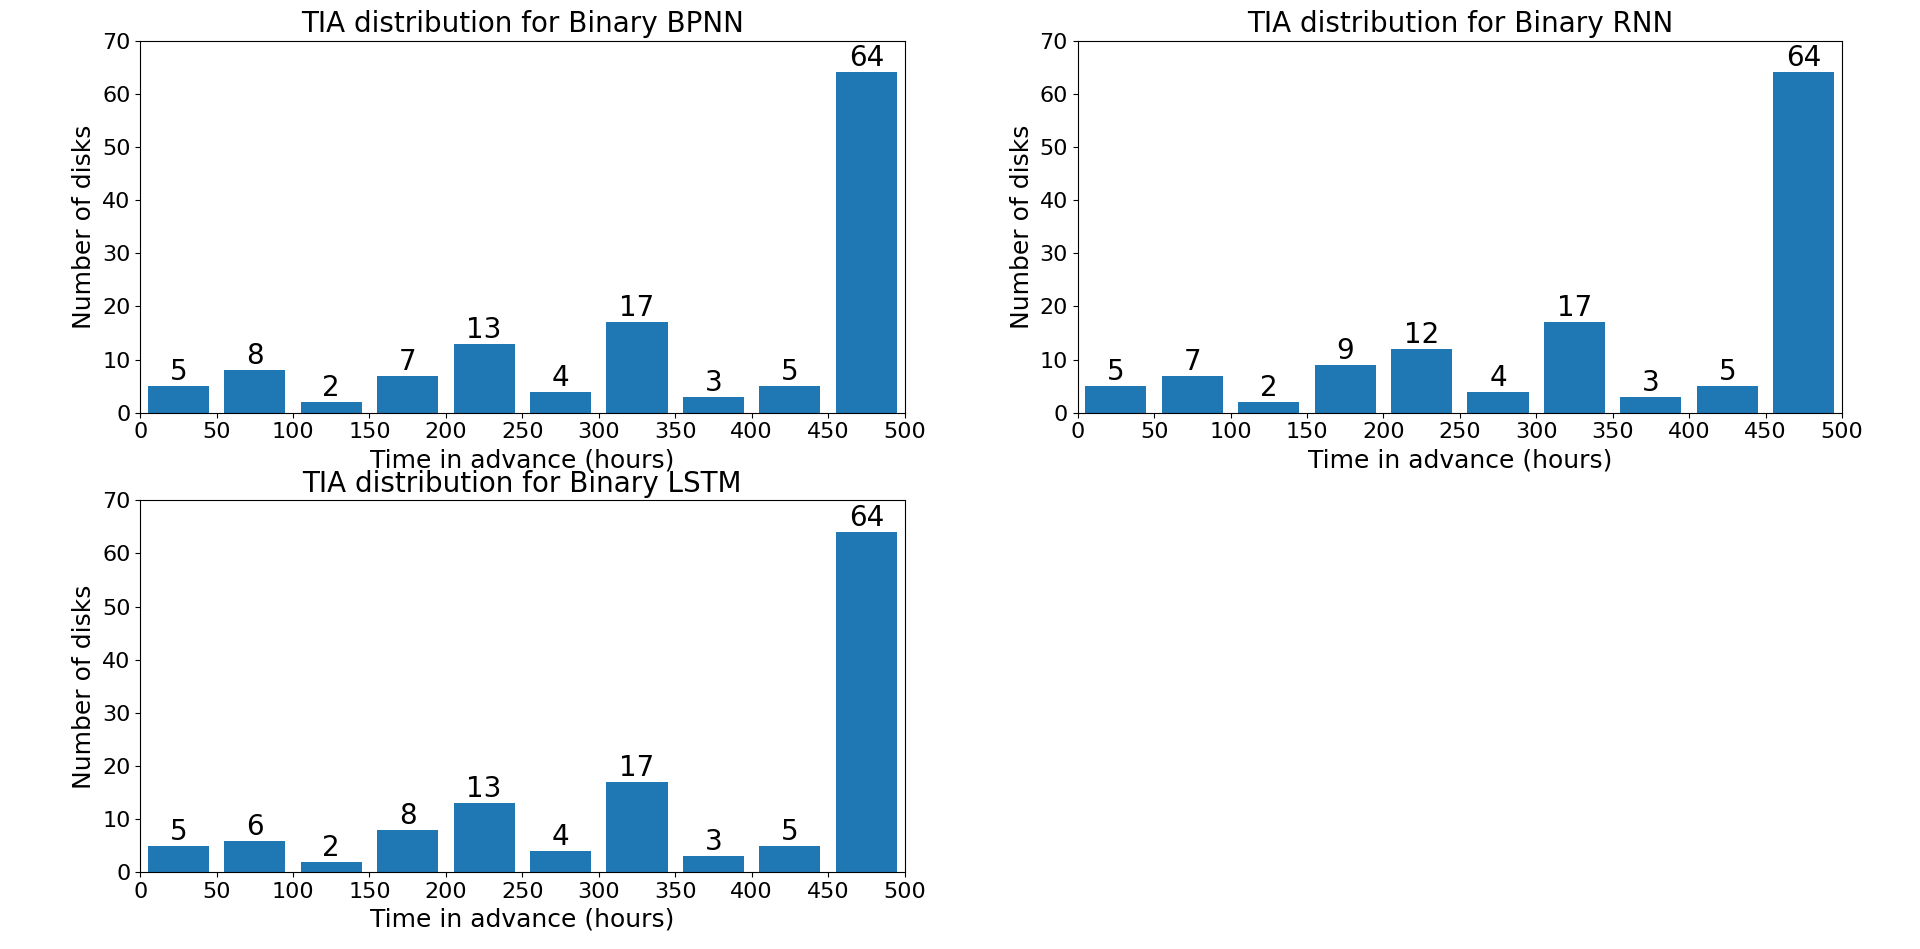
\includegraphics[width=1.0\linewidth]{TIA_Binary_Networks.png}
  \caption[TIA for binary networks]{Time In Advance distribution for binary networks}
  \label{fig:tia_binary_network}
\end{center}
\end{figure}

\begin{figure}
\begin{center}
  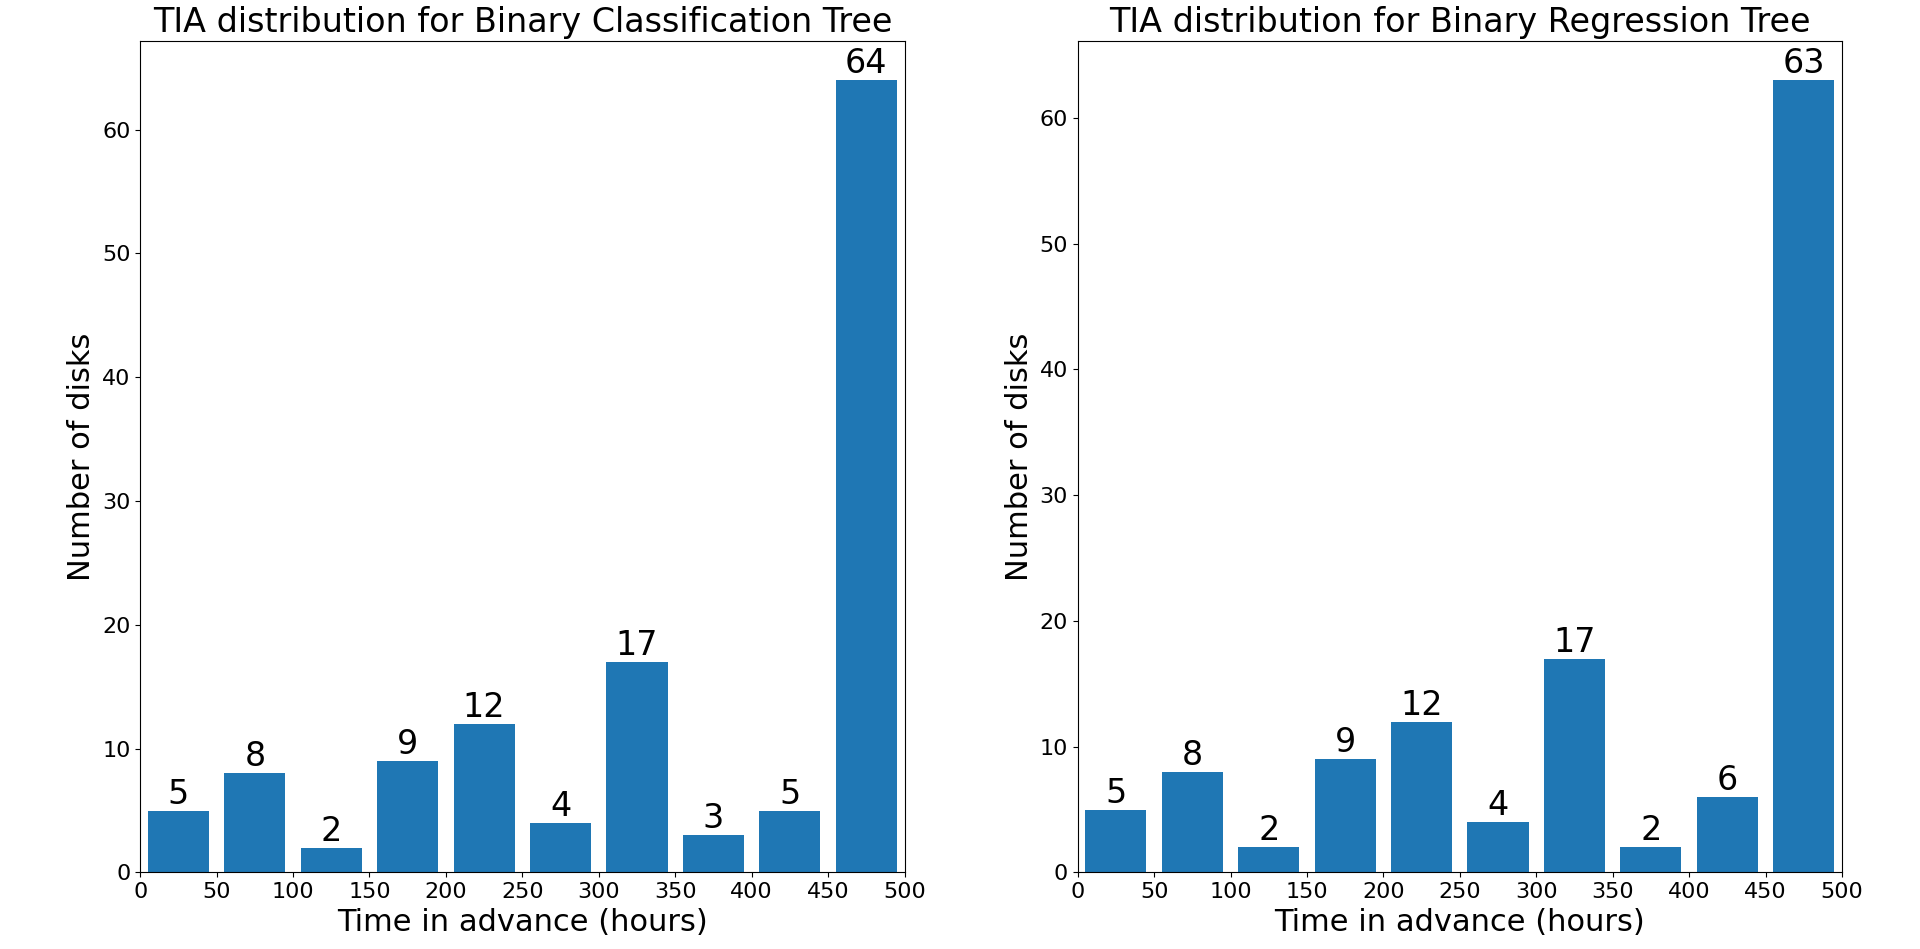
\includegraphics[width=0.9\linewidth]{TIA_Binary_Trees.png}
  \caption[TIA for binary decision trees]{Time In Advance distribution for binary decision trees}
  \label{fig:tia_binary_tree}
\end{center}
\end{figure}

The analysis we can make of these results is firstly that the three network models behave similarly.
LSTM is a little better than the RNN, which is a little better than BPNN.

However, the fact that the three achieve the same FDR indicates that the disks they cannot correctly classify is due more to the nature of the problem than to incorrect hyperparameters.
The cause of these failures that none of the models could predict may be some events that cannot be monitored using SMART attributes such as current surges.

The classification tree performs better than any of the network based models and is only beaten by the regression tree.
This indicates that these older, simpler models are still very powerful and should not be overlooked.

The distribution of the TIA for the different models signals that all of them are capable of detecting signals of problems hundreds of hours in advance
In practical terms, this means that the people responsible for managing the datacenters will have plenty of time to swap the failing disks and prevent any data loss or disruption of service.

The smallest value of the TIA for every model was 19 hours.
This implies that no rushing is needed when a failure is predicted.
The main risk lies instead on the disks that have not been detected.

The capacity of such models to be highly sensitive to failing disks in order to detect problems much before they occur while keeping an FAR below 2\% proves that all of them are powerful methods to tackle the problem at hand.

Concerning the time to train and test the models, we have the Classification Trees being the fastest ones to train, taking 2 minutes on average.
The BPNN also takes a very short time, around 4 minutes.

The RNN and LSTM take a little longer: on average 8 minutes.
This is due to the fact that these are time sensitive models and therefore the samples must be evaluated in order.
This reduces the capabilities of the model to perform tasks in parallel.

All experiments have been performed on an ordinary desktop computer, with an AMD Ryzen 5 5560U CPU.
No GPU acceleration was needed.

We can compare our results to other experiments performed on the same dataset in \cite{Zhu13}.
Our results are similar to theirs, who obtained a better FAR of 1.14\% but a slightly worse FDR of 97.69\%.

The advantage of our approach is that we can directly compare the performance of different models without introducing bias due to different datasets or different preprocessing steps.

On the next few pages we will describe the impact of the feature selection algorithms as well as how the voting process can improve the results.
Finally, we will show that the inclusion of the change rates of the SMART attributes improves the performance of every model.

\subsection{Feature Selection Algorithms}

We have trained our different models using the different feature selection algorithms described on Subsection \ref{subsec:feature_selection}.
We still used the default parameters presented on Appendix \ref{chap:config_files}, with the only modifications being on the \verb|feature_count| that was set to 15 and, of course, on \verb|feature_selection_algorithm|.
The results are displayed on Figure \ref{fig:fs_binary}.

\begin{figure}
\begin{center}
  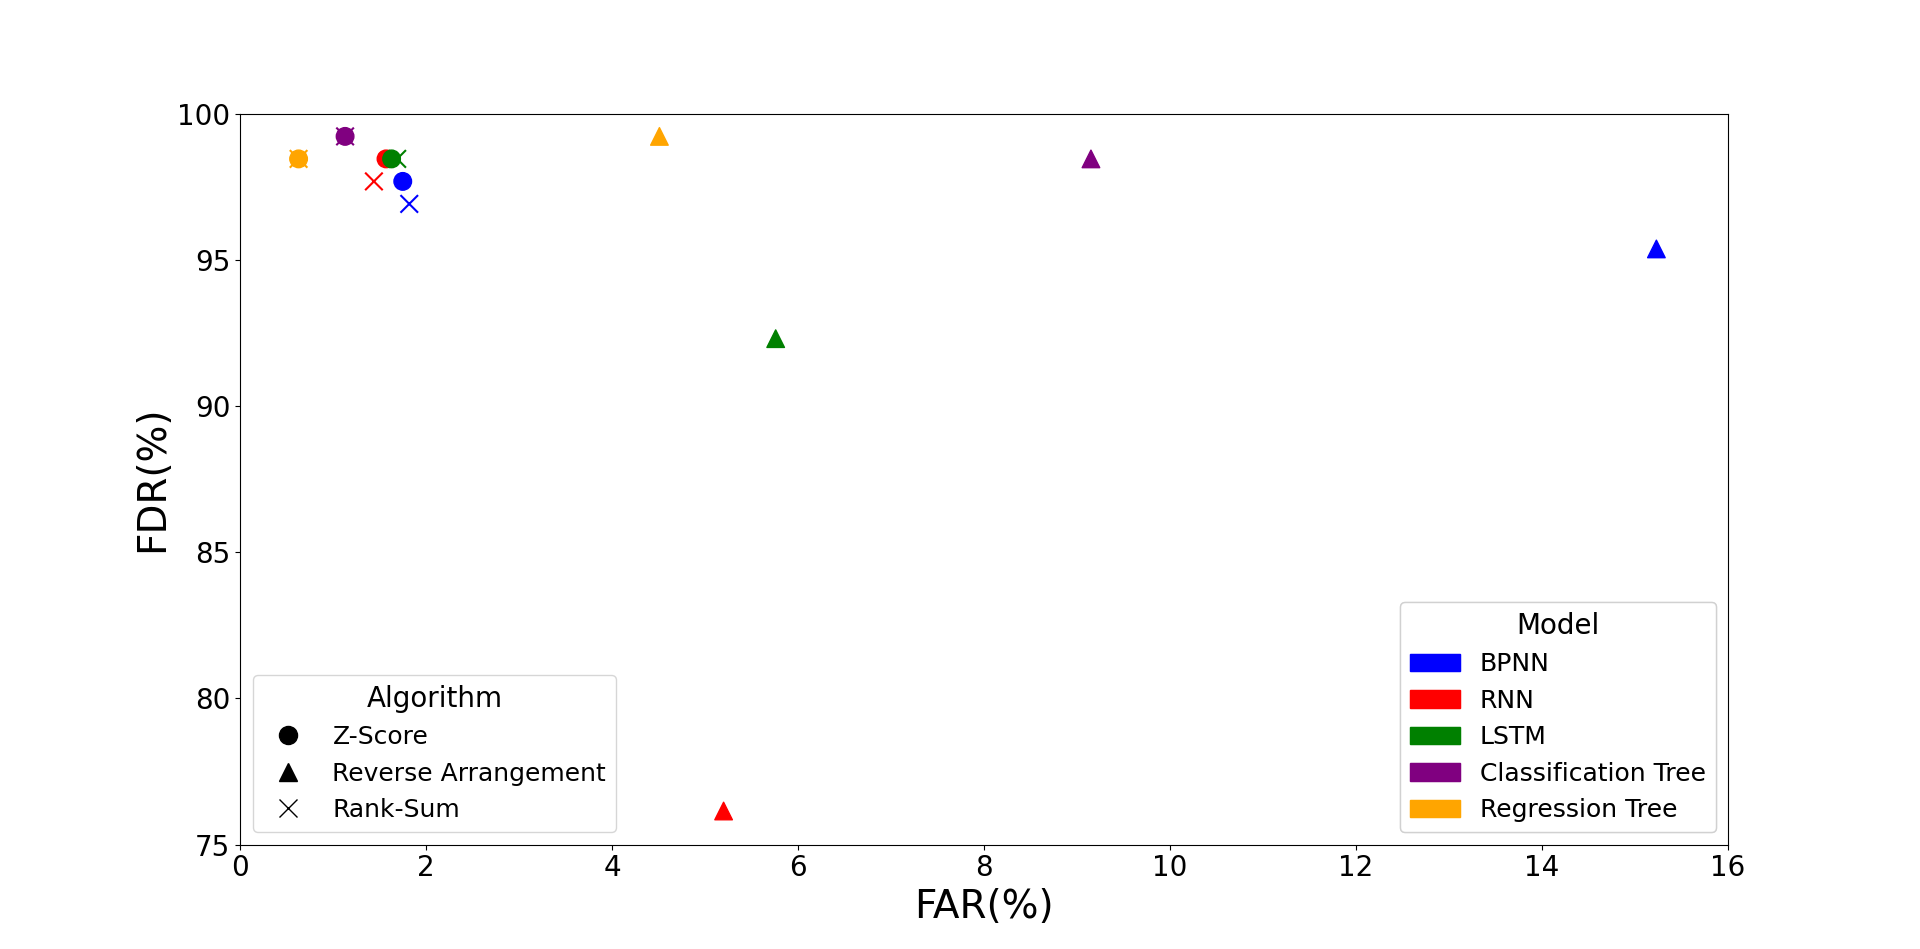
\includegraphics[width=1.0\linewidth]{FS_Binary.png}
  \caption[Feature Selection Results]{Results for different feature selection algorithms for binary models for Feature Count = 15}
  \label{fig:fs_binary}
\end{center}
\end{figure}

The most striking pattern we can observe is that the Reverse Arrangement algorithm had a worse performance than the other two on all scenarios we have tested.

Moreover, the Z-Score algorithm is slightly better than the Rank-Sum test for the network-based models.
However, the result of these two algorithms is the same for our decision trees.

If we observe which features are kept by the three algorithms, we see that 11 of them are common to all of them.
These are features such as Reallocated Sector Count, Temperature and Seek Error Rate, which is to be expected since these can easily indicate failure.

Surprisingly, between the Rank-Sum and the Reverse Arrangement algorithms, only 3 of the 15 features change, but this is already enough to generate completely different results.
Two of the features that appear in the selection done by the Reverse Arrangement but do not appear on Rank-Sum one are change rate features: the Current Pending Sector Change Rate and the Seek Error Rate Change Rate.
The third one, High Fly Writes, also do not appear in the Z-Score selection.

This indicates that the change rate features allow the models to learn the classification problem more efficiently.
We will explore this further on Subsection \ref{subsec:change_rate_impact}.

\subsection{Voting}

To observe how the voting process can influence the performance of the models, we ran our experiments with the default configuration but using 7 votes instead of only 1.
We still kept the vote threshold at 0.5.
As discussed on Subsection \ref{subsec:voting}, for the binary models we are presenting, only the Class Based Voting Algorithm can be used.

The results of this experiment are displayed on Table \ref{table:results_binary_voting}. 

\begin{table}
  \begin{center}
    \begin{tabular}{|c|c|c|c|c|}
      \hline
    Model & FAR(\%) & FDR(\%) & TIA(h) & TIA SD(h) \\
    \hline
    BPNN & 1.63 & 96.15 & 366.0 & 145.0 \\
    RNN & 1.63 & 99.23 & 375.3 & 137.7 \\
    LSTM & 1.13 & 98.46 & 362.7 & 145.6\\
    Classification Tree & 1.13 & 99.23 & 359.8 & 147.7 \\
    Regression Tree & 1.13 & 99.23 & 341.0 & 154.2 \\
    \hline
    \end{tabular}
    \caption[Results Binary Models with Voting]{Results for binary models with Vote Count set to 7}
    \label{table:results_binary_voting}
  \end{center}
\end{table}

As we can see, the results are very similar to the original ones.
For the RNN model, there was a slight decrease on the FAR.
For the Regression Tree, the FDR decreased a bit and became equal to the ones for the network based models.

Moreover, on all models the TIA decreased a little bit.
This was expected due to the fact that now more than one sample is not enough to classify a disk as failing.

The fact that the FDR didn't change a lot was to be expected given the results displayed on Figures \ref{fig:tia_binary_network} and \ref{fig:tia_binary_tree}.
Usually, a failing disk will start producing samples indicating it much before it crashes.

Therefore, the probability that a sequence with many samples that can be predicted as failing is high.
Thus, the decrease of the FDR is expected to be small, which is the result we obtained.

For the LSTM, we obtained a result that at first seem counterintuitive.
Even though with 7 votes more than one sample needs to be classified as bad in order to flag the disk as failing, we obtained a smaller FAR.
In other words, the number of disks flagged as failing was strictly smaller.

But this is due to the method we use to do the voting.
Since, as explained in section \ref{subsec:voting}, with more votes a longer sequence is passed to the LSTM at once, with more than one vote, it is able to apply its ability to learn sequences.

So the result we observed actually shows the main advantage of the time sensitive models: they take the context into account.


Now, if we keep the vote count to 7 but increase the vote threshold to 0.8, we obtain the results shown on Table \ref{table:results_binary_threshold}.

\begin{table}
  \begin{center}
    \begin{tabular}{|c|c|c|c|c|}
      \hline
    Model & FAR(\%) & FDR(\%) & TIA(h) & TIA SD(h) \\
    \hline
    BPNN & 1.63 & 96.15 & 366.0 & 145.1 \\
    RNN & 1.63 & 99.23 & 375.3 & 137.7 \\
    LSTM & 0.81 & 98.46 & 362.5 & 146.0 \\
    Classification Tree & 1.13 & 99.23 & 359.7 & 147.7 \\
    Regression Tree & 0.69 & 98.46 & 342.8 & 152.9 \\
    \hline
    \end{tabular}
    \caption[Results Binary Models with Threshold]{Results for binary models with Vote Count set to 7 and Vote Threshold equal to 0.8}
    \label{table:results_binary_threshold}
  \end{center}
\end{table}

Again we observe a further decrease on the value of the FAR, the FDR and the TIA for some models.
The Regression Tree is able to achieve an FAR as small as 0.56\% which is the smallest value we found for it.

The most interesting approach of using a voting algorithm is that the value of the vote count and threshold can be modified without needing to retrain the model, which is not the case when changing the feature count or the feature selection algorithm.
Therefore, voting is a powerful and fast to use tool to fine tune the FAR-FDR trade off.

\subsection{Change Rate Impact}\label{subsec:change_rate_impact}

The next step was to observe how including the change rate of the original SMART attributes affects the performance of our models.
So, we trained our models without computing the change rates.
In order to remove any impact due to feature selection algorithms, we used all 12 SMART attributes.

The results are displayed on table \ref{table:results_binary_no_change_rate}

\begin{table}
  \begin{center}
    \begin{tabular}{|c|c|c|c|c|}
      \hline
    Model & FAR(\%) & FDR(\%) & TIA(h) & TIA SD(h) \\
    \hline
    BPNN & 2.13 & 98.46 & 363.7 & 145.1 \\
    RNN & 1.57 & 98.46 & 357.4 & 145.9 \\
    LSTM & 2.07 & 95.38 & 361.8 & 143.6 \\
    Classification Tree & 1.07 & 99.23 & 354.7 & 147.8 \\
    Regression Tree & 1.07 & 97.69 & 354.7 & 147.8 \\
    \hline
    \end{tabular}
    \caption[Results Binary Models with Voting]{Results for binary models with Vote Count set to 7}
    \label{table:results_binary_no_change_rate}
  \end{center}
\end{table}

Most notably, every model had a worse performance compared to the original version using the change rates.
This shows that the change rate we computed carries information than can be used by the models to better learn the problem.

Moreover, it is interesting to see that the models that had the best performance were the two Decision Tree ones with information about the change rates.
The fact that they both Classification and Regression Trees are time insensitive implies that we can encode useful information about the problem in the form of change rates. 

\section{Multiclass Models}

The next step is to inverstigate the behavior of the multiclass models.
Their hyperparameters are listed on Appendix \ref{chap:config_files}.
Most importantly, we used as a base value a Health Status Count of 4.

The results of our experiment are displayed on Tables \ref{table:results_multiclass_score_one_vote} and \ref{table:results_multiclass_class_one_vote}, presenting the performance of the models when using the Score and Class Based Voting Algorithms respectively.
All experiments were performed with a Health Status Count of 4 and a vote count of one.

Some modification on the hyperparameters were needed when compared to the binary models.
For the Regression Tree, for instance, the maximum depth of the tree had to be increased to 15.

Moreover, for the RNN and the LSTM models, the number of failing samples had to be increased to 96 to obtain a better granularity of the training samples corresponding to each class.
This impacted the time required to train these models, but it was still around 40 minutes in an ordinary desktop computer's CPU, which is still manageable.

\begin{table}
  \begin{center}
    \begin{tabular}{|c|c|c|c|c|}
      \hline
    Model & FAR(\%) & FDR(\%) & TIA(h) & TIA SD(h) \\
    \hline
    BPNN & 1.63 & 95.38 & 359.3 & 144.9 \\
    RNN & 3.57 & 94.62 & 375.9 & 134.7 \\
    LSTM & 1.94 & 97.69 & 358.4 & 142.9 \\
    Classification Tree & 1.25 & 96.92 & 347.7 & 144.1 \\
    Regression Tree & 0.75 & 99.23 & 353.0 & 147.8 \\
    \hline
    \end{tabular}
    \caption[Results Multiclass Models, Score Voting, 1 vote]{Results for multiclass models with Score Based Voting(1 vote)}
    \label{table:results_multiclass_score_one_vote}
  \end{center}
\end{table}

\begin{table}
  \begin{center}
    \begin{tabular}{|c|c|c|c|c|}
      \hline
    Model & FAR(\%) & FDR(\%) & TIA(h) & TIA SD(h) \\
    \hline
    BPNN & 1.50 & 95.38 & 359.7 & 142.3 \\
    RNN & 1.32 & 96.92 & 355.1 & 145.5 \\
    LSTM & 1.88 & 97.69 & 354.2 & 146.7 \\
    Regression Tree & 1.13 & 99.23 & 346.5 & 149.1 \\
    \hline
    \end{tabular}
    \caption[Results Multiclass Models, Class Voting, 1 vote]{Results for multiclass models with Class Based Voting (1 vote)}
    \label{table:results_multiclass_class_one_vote}
  \end{center}
\end{table}

The results show that most multiclass models do not perform as well as their binary counterparts.
The main exception being, of course, the Regression Tree model with Score Based Voting which is able to keep the same FDR with a smaller FAR than its binary version.

If we compare the impact of the two voting algorithms, we observe that most models have a better performance using Class Based Voting for this scenario of using a Vote Count equal to 1.

Our results conflict with the ones presented by \cite{Xu16} which concluded that multiclass RNNs are the most performant models.
This can be due multiple factors.

Firstly, the datasets are not the same, as we only have access to a subset of the dataset used in \cite{Zhu13}.
Secondly, the results we obtained for the three models we implemented that they also tested are much better than the ones they found.
These three models are the binary and multiclass BPNN as well as the Classification Tree.

This fact indicates that we made a more unbiased exploration and comparison of the different models.
These results show the importance of the current work of more impartially comparing different models instead of trying to prove that a specific one is more powerful than others.

\subsection{Voting}

In order to evaluate our proposed voting algorithm and compare it with the other one already present in literature, we performed the experiments now using a vote count equal to 7.
The results obtained using the Score Based Voting Algorithm and the Class Based one are shown on Tables \ref{table:results_multiclass_score_multi_vote} and \ref{table:results_multiclass_class_multi_vote} respectively.

\begin{table}
  \begin{center}
    \begin{tabular}{|c|c|c|c|c|}
      \hline
    Model & FAR(\%) & FDR(\%) & TIA(h) & TIA SD(h) \\
    \hline
    BPNN & 1.57 & 95.38 & 366.3 & 142.4 \\
    RNN & 4.51 & 96.15 & 342.9 & 154.3 \\
    LSTM & 5.33 & 99.23 & 377.1 & 135.5 \\
    Regression Tree & 0.63 & 99.23 & 359.1 & 147.7 \\
    \hline
    \end{tabular}
    \caption[Results Multiclass Models, Score Voting, 7 votes]{Results for multiclass models with Score Based Voting(7 votes)}
    \label{table:results_multiclass_score_multi_vote}
  \end{center}
\end{table}

\begin{table}
  \begin{center}
    \begin{tabular}{|c|c|c|c|c|}
      \hline
    Model & FAR(\%) & FDR(\%) & TIA(h) & TIA SD(h) \\
    \hline
    BPNN & 1.50 & 95.38 & 365.7 & 142.0 \\
    RNN & 1.32 & 98.46 & 362.1 & 145.7 \\
    LSTM & 4.70 & 99.23 & 377.1 & 135.5\\
    Classification Tree & 5.33 & 99.23 & 377.1 & 135.5 \\
    Regression Tree & 0.69 & 99.23 & 359.2 & 147.4 \\
    \hline
    \end{tabular}
    \caption[Results Multiclass Models, Class Voting, 7 votes]{Results for multiclass models with Class Based Voting(7 votes)}
    \label{table:results_multiclass_class_multi_vote}
  \end{center}
\end{table}

For the Score Voting, we omit the results for the Classification Tree model.
This is due to the fact that, for a Classification Tree, no score is assigned and therefore the Score Based Voting Algorithm cannot be applied.

If we observe the results and compare to the results in Tables \ref{table:results_multiclass_score_one_vote} and \ref{table:results_multiclass_class_one_vote} which use a vote count equal to 1, we observe different behaviors.
The BPNN kept the same FDR but obtained a smaller FAR.
The FAR when using Class Based Voting was slightly smaller.

For the LSTM and Classification Tree, the FDR was improved, although the FAR increased by a noticeable amount.

The RNN in particular improved the most by using the Class Based Voting.
It achieved a better FAR and FDR than either the version using one vote and the one with 7 votes and Score Based Voting.

The Regression Tree model was able to keep a great FDR equivalent to the best values we have obtained over all models we have explored.
At the same time, increasing the number of votes decreased the FAR, with our proposed Score Based Voting obtaining the smallest FAR.

\subsection{Health Status Count}

During our experiments, we noticed that increasing the number of different classed to 5 or 6 resulted in patterns that were more difficult for our models to learn.
Specially for the RNN and LSTM models, the result of the experiment was highly dependent on the fine tuning of hyperparameters as well as on the seed used.

This is mainly due to the fact that when increasing the Health Status Count there are two possible scenarios.
The first is that we decrease the number of samples per class.
The only way to mitigate this is to increase the Number of Failing Samples, which results in the training set having less relevant samples since they will be taken far away from the critical moment of failure.

Either way, it may make it more difficult for our models to learn to predict failures.
Indeed, we observe that for a Health Status Count of 3 or 4, our models are still able to perform well.
On the other hand,  for a higher number of classes, the effects mentioned on the last paragraph override the benefits we gain by interpreting the problem from a multiclass point of view.

% TODO: include the other voting algorithm

On Table \ref{table:results_multiclass_three_health_status} we display the results of our experiments when Health Status Count is set to 3.

\begin{table}
  \begin{center}
    \begin{tabular}{|c|c|c|c|c|}
      \hline
    Model & FAR(\%) & FDR(\%) & TIA(h) & TIA SD(h) \\
    \hline
    BPNN & 1.69 & 96.92 & 358.6 & 144.5 \\
    RNN & 1.32 & 98.46 & 368.3 & 138.6 \\ 
    LSTM & 1.82 & 98.46 & 356.1 & 142.9\\
    Classification Tree & 1.57 & 96.92 & 352.4 & 139.3 \\
    Regression Tree & 1.63 & 97.69 & 350.3 & 146.6 \\
    \hline
    \end{tabular}
    \caption[Results Multiclass Models with Health Status Count set to 3]{Results for Multiclass Models with Health Status Count set to 3}
    \label{table:results_multiclass_three_health_status}
  \end{center}
\end{table}

For the network based models, reducing the Health Status Count caused an improvement when compared to the approach of using 4 Health Status as depicted on Tables \ref{table:results_multiclass_score_one_vote} and \ref{table:results_multiclass_score_multi_vote}.
In the case of the RNN specifically, it achieved a FAR smaller than its binary counterpart, with the trade off being a slight worse FDR that is still acceptably high.

This shows the power of our approach of generalizing the problem to use more than two classes.

In contrast, the Decision Tree Models performed better with a Health Status Count equal to 4.

For every model, the performance increases up to some value of Health Status Count and then starts decreasing.
This value can different for each one.

This implies that the models' performance are highly sensitive to the value of Health Status Count.
However, given that the ideal value is a small integer number, it is not very difficult to explore the space of possibilities to find the best one.
\chapter{Discussion}\label{chap:discussion}


Discuss the results. What is the outcome of your experiments?
\chapter{Conclusion}\label{chap:conclusion}

In the present work, the hard drive failure prediction problem has been explored.
More specifically we tackled the challenge to use SMART attributes to make our predictions.

We started by discussing the main approaches possible to tackle the problem.
Firstly, we explored the possibilities from treating it from a binary classification point of view.
This allows us to use different models such as Decision Trees and the naive backpropagation neural network.

However, by noticing that the samples available for each disk form is a time series, we were able to use some additional approaches.

Firstly, we proposed the use of recurrent neural networks and long short-term memory.
These are models that have been designed with the objective of learning sequences, including time series which is our use case.

Then, we took advantage of the fact that we are using time series to make use of the concept of health status.
We can notice that not every sample coming from a failing disk is made equal, we actually expect the ones closer to the point of failure to present a different profile from the ones taken long before this critical time.
Therefore, we can divide our samples coming from failing disks in different classes.

This multiclass approach allows us to extend our models.
We created generalizations of each one of our five models to be able to tackle the multiclass version of the problem.

Since, in the end, we still want to classify the disks outside the training set in only two classes, some additional tools were needed.
More specifically, we developed some voting algorithms to translate the results from our multiple classes into only two of them.

During our experiments, we have explored the impact of different hyperparameters on the performance of the models.
We have shown that not only these models are able to correctly identify healthy and failing disks, but they are also able to alert for failures much before it actually happens.

This last part is important because in a real world scenario some actions have to be taken to ensure that the data saved in the disk is not lost.

Moreover, we have implemented and studied the entire pipeline needed to tackle the problem.
So we also studied the impact of some steps such as the feature selection algorithm, the inclusion of the change rates and the voting algorithm.

This was made possible thanks to the implementation of a library capable of performing all the steps from reading the dataset to evaluating the performance of all of our models.
Our code treats each different step as an independent module and therefore the impact of the different steps and hyperparameters could be observed separately.

This report, together with our code, intends to be a reference to the hard drive failure prediction problem.
Therefore, we compiled a set of different possible approaches and the theory behind them, we explained the steps taken to tackle the problem, and we provide an implementation.

One of the main improvements produced by our work is to try to make an unbiased evaluation of the different models, some already present in the literature and others not.
By using the same pre and post-processing steps, as well as the same dataset we remove most sources of bias.

Moreover, we do not try to prove that a specific model is better.
So, we show that most models have similar performances.

In literature, we often find that the model being introduced is much better than the others. 
However, by implementing these same models and testing them on the same dataset we have shown that this is not always the case.
This disparity is probably caused in most cases due to spending more time fine-tuning the novel model.

Finally, as far as we know, ours is the first implementation of LSTMs with SMART attributes to tackle the problem at hand that can be compared to other works.

This is due to the fact that the only other implementation we have found, by \cite{zhang2017deep}, was concerned with introducing an event detection approach.
Therefore, the metrics they used were different, and they were observing the impact of only their proposed method rather than exploring all the hyperparameters to obtain the best FAR and FDR possible.

Future work with the problem should be concerned, firstly, with exploring the performance of the models for different datasets, since most of them are proprietary.

We have shown that the given models are able to learn to identify the required patterns.
However, since results can vary for different models of disks, we cannot know exactly how each model will perform and, specially, we cannot guarantee that the hyperparameters will be the same at all.

This discrepancy that can exist for different datasets was one of the main motivations for creating the current work, which gathers different models to the problem.

Another avenue to improve the understanding of the problem is to use models other than ours, such as support vector machines or convolutional neural networks.
The objective of developing our library was exactly to allow other models to be implemented and to be objectively compared to others.

Also, modifying the voting or feature selection processes can impact the outcomes as we have shown.
Therefore, improving them can be another path to obtain even better results.

% -- Appendix (optional)
% \begin{appendices}
%     % !TeX spellcheck = en_US
% !TeX encoding = UTF-8
\chapter{Configuration Files}\label{chap:config_files}

Below we have the standard configurations for each of the models we trained.
When mentioning the results, if the value of a parameter is not mentioned, then it is because the value indicated below is used.

\begin{lstlisting}[language=Toml,caption={Default configuration file for a Binary BPNN}]
[dataset]
seed = 0
data_file = "data/baidu-dataset.csv"
number_of_failing_samples = 12

[preprocessing]
change_rate_interval = 1
feature_count = 19
feature_selection_algorithm = "z_score"
health_status_algorithm = "discrete"
good_bad_ratio = 0.6

[model]
model_type = "NN"
model = "BinaryBPNN"
health_status_count = 2
hidden_nodes = 30
epoch_count = 1500
learning_rate = 0.1
evaluate_interval = 1500
lr_decay_interval = 100000

[vote]
vote_count = 1
vote_threshold = 0.5
\end{lstlisting}

\newpage

\begin{lstlisting}[language=Toml,caption={Default configuration file for a Binary RNN}]
[dataset]
seed = 0
data_file = "data/baidu-dataset.csv"
number_of_failing_samples = 12

[preprocessing]
change_rate_interval = 1
feature_count = 19
feature_selection_algorithm = "z_score"
health_status_algorithm = "discrete"
good_bad_ratio = 20.0

[model]
model_type = "NN"
model = "BinaryRNN"
health_status_count = 2
hidden_nodes = 10
epoch_count = 700
learning_rate = 0.1
evaluate_interval = 700
lr_decay_interval = 100
lookback = 6

[vote]
vote_count = 1
vote_threshold = 0.5
\end{lstlisting}

\begin{lstlisting}[language=Toml,caption={Default configuration file for a Binary LSTM}]
[dataset]
seed = 0
data_file = "data/baidu-dataset.csv"
number_of_failing_samples = 12

[preprocessing]
change_rate_interval = 1
feature_count = 19
feature_selection_algorithm = "z_score"
health_status_algorithm = "discrete"
good_bad_ratio = 15.0

[model]
model_type = "NN"
model = "BinaryLSTM"
health_status_count = 2
hidden_nodes = 10
epoch_count = 700
learning_rate = 0.1
evaluate_interval = 700
lr_decay_interval = 100
lookback = 6

[vote]
vote_count = 1
vote_threshold = 0.5
\end{lstlisting}

\begin{lstlisting}[language=Toml,caption={Default configuration file for a Multiclass-Level BPNN}]
[dataset]
seed = 0
data_file = "data/baidu-dataset.csv"
number_of_failing_samples = 12

[preprocessing]
change_rate_interval = 1
feature_count = 19
feature_selection_algorithm = "z_score"
health_status_algorithm = "discrete"
good_bad_ratio = 0.6

[model]
model_type = "NN"
model = "MultiLevelBPNN"
health_status_count = 4
hidden_nodes = 30
epoch_count = 1500
learning_rate = 0.1
evaluate_interval = 1500
lr_decay_interval = 100000

[vote]
vote_count = 1
vote_threshold = 0.5
\end{lstlisting}

\begin{lstlisting}[language=Toml,caption={Default configuration file for a Multiclass RNN}]
[dataset]
seed = 0
data_file = "data/baidu-dataset.csv"
number_of_failing_samples = 12

[preprocessing]
change_rate_interval = 1
feature_count = 19
feature_selection_algorithm = "z_score"
health_status_algorithm = "discrete"
good_bad_ratio = 20.0

[model]
model_type = "NN"
model = "MultiLevelRNN"
health_status_count = 4
hidden_nodes = 10
epoch_count = 700
learning_rate = 0.1
evaluate_interval = 700
lr_decay_interval = 100
lookback = 6

[vote]
vote_count = 1
vote_threshold = 0.5
\end{lstlisting}

\begin{lstlisting}[language=Toml,caption={Default configuration file for a Multiclass LSTM}]
[dataset]
seed = 0
data_file = "data/baidu-dataset.csv"
number_of_failing_samples = 12

[preprocessing]
change_rate_interval = 1
feature_count = 19
feature_selection_algorithm = "z_score"
health_status_algorithm = "discrete"
good_bad_ratio = 10.0

[model]
model_type = "NN"
model = "MultiLevelLSTM"
health_status_count = 4
hidden_nodes = 10
epoch_count = 700
learning_rate = 0.1
evaluate_interval = 700
lr_decay_interval = 100
lookback = 6

[vote]
vote_count = 1
vote_threshold = 0.5
\end{lstlisting}

\begin{lstlisting}[language=Toml,caption={Default configuration file for a Classification Tree}]
[dataset]
seed = 0
data_file = "data/baidu-dataset.csv"
number_of_failing_samples = 12

[preprocessing]
change_rate_interval = 1
feature_count = 19
feature_selection_algorithm = "z_score"
health_status_algorithm = "discrete"
good_bad_ratio = 0.6

[model]
model_type = "TREE"
tree_type = "CLASSIFICATION"
health_status_count = 2
criterion = "GINI"
max_depth = 5
min_samples_leaf = 5

[vote]
vote_count = 1
vote_threshold = 0.5
\end{lstlisting}

\begin{lstlisting}[language=Toml,caption={Default configuration file for a Regression Tree}]
[dataset]
seed = 0
data_file = "data/baidu-dataset.csv"
number_of_failing_samples = 12

[preprocessing]
change_rate_interval = 1
feature_count = 19
feature_selection_algorithm = "z_score"
health_status_algorithm = "continuous"
good_bad_ratio = 1.0

[model]
model_type = "TREE"
tree_type = "REGRESSION"
health_status_count = 2
criterion = "SQUARED_ERROR"
max_depth = 5
min_samples_leaf = 5

[vote]
vote_count = 1
vote_threshold = 0.5
\end{lstlisting}
% \end{appendices}
% \newpage


%%%%%%%%%%%%%%%%%%%%%%%%%%%%%%%%%%%%%%%%%%%%%%%%%%%%%%%%%%%%%%%%%%%%%%%%%%%%%%%%%%%%%%%%%
\backmatter

% -- Bibliography
\printbibliography

% -- Eidesstattliche Erklärung (= Affadavit)
% !TeX spellcheck = de_DE
% !TeX encoding = UTF-8

\chapter{Eidesstattliche Erkl\"arung}

	Hiermit versichere ich, dass ich diese \thesisType{} selbstst\"andig und ohne Benutzung anderer als der angegebenen Quellen und Hilfsmittel angefertigt habe und alle Ausf\"uhrungen, die w\"ortlich oder sinngem\"a\ss{} übernommen wurden, als solche gekennzeichnet sind, sowie, dass ich die \thesisType ~in gleicher oder \"ahnlicher Form noch keiner anderen Pr\"ufungsbeh\"orde vorgelegt habe.

	\vspace{3cm}

	Passau, \thedate

	\vspace{2cm}

	\parbox{8cm}{
		\hrule \strut \theauthor
	}




\end{document}